% !TeX encoding = UTF-8
% !TeX program = xelatex
% !TeX spellcheck = en_US

\documentclass[degree=doctor]{thuthesis}
  % 学位 degree:
  %   doctor | master | bachelor | postdoc
  % 学位类型 degree-type:
  %   academic(默认)| professional


% 论文基本配置,加载宏包等全局配置
% !TeX root = ./thuthesis-example.tex
% Settings for basic information of thesis
% 论文基本信息配置

\thusetup{
  %******************************
  % 注意:
  %   1. 配置里面不要出现空行
  %   2. 不需要的配置信息可以删除
  %   3. 建议先阅读文档中所有关于选项的说明
  %******************************
  %
  % 输出格式
  %   选择打印版(print)或用于提交的电子版(electronic),前者会插入空白页以便直接双面打印
  %
  output = print,
  degree=master,
  language=english,
  % 标题
  %   可使用“\\”命令手动控制换行
  %
  % Input your title in CHINESE & English: 
  title  = {针对于物联网环境研究之下的真实-虚拟世界连接界面\\
  \textbf{Real-virtual world connection interface for research in IoT environment}},
  % Input your title* in ENGLISH
  title* = {Real-virtual world connection interface for research in IoT environment},
  %
  % 学位
  %   1. 学术型
  %      - 中文
  %        需注明所属的学科门类,例如:
  %        哲学、经济学、法学、教育学、文学、历史学、理学、工学、农学、医学、
  %        军事学、管理学、艺术学
  %      - 英文
  %        博士:Doctor of Philosophy
  %        硕士:
  %          哲学、文学、历史学、法学、教育学、艺术学门类,公共管理学科
  %          填写“Master of Arts“,其它填写“Master of Science”
  %   2. 专业型
  %      直接填写专业学位的名称,例如:
  %      教育博士、工程硕士等
  %      Doctor of Education, Master of Engineering
  %   3. 本科生不需要填写
  %
  % Please do no change:
  degree-name  = {工学硕士},
  degree-name* = {Master of Science},
  %
  % 培养单位
  %   填写所属院系的全名
  %
  department = {计算机科学与技术系},
  %
  % 学科
  %   1. 学术型学位
  %      获得一级学科授权的学科填写一级学科名称,其他填写二级学科名称
  %   2. 工程硕士
  %      工程领域名称
  %   3. 其他专业型学位
  %      不填写此项
  %   4. 本科生填写专业名称,第二学位论文需标注“(第二学位)”
  %
  discipline  = {计算机科学与技术},
  discipline* = {Computer Science and Technology},
  %
  % 姓名
  %
  % Please input your full name in CHINESE
  author  = {费杰},
  % Please input your full name in ENGLISH
  author* = {Ivachev Fedor},
  %
  % 指导教师
  %   中文姓名和职称之间以英文逗号“,”分开,下同
  %
  % Please input your supervisor's full name in Chinese, then comma, followed by 教授 (for Professor) and 副教授 (for Associate Prof.)
  supervisor  = {喻纯, 副研究员},
  % Please input your supervisor's title (ie Professor) and followed by full name in English
  supervisor* = {Associate Professor Yu Chun},
  %
  % 副指导教师
  %
  % associate-supervisor  = {陈文光, 教授},
  % associate-supervisor* = {Professor Chen Wenguang},
  %
  % 联合指导教师
  %
  % joint-supervisor  = {某某某, 教授},
  % joint-supervisor* = {Professor Mou Moumou},
  %
  % 日期
  %   使用 ISO 格式;默认为当前时间
  %
  % Please change the date as required
  date = {2021-04-15},
  %
  % 是否在中文封面后的空白页生成书脊(默认 false)
  %
  include-spine = false,
  %
  % 密级和年限
  %   秘密, 机密, 绝密
  %
  % secret-level = {秘密},
  % secret-year  = {10},
  %
  % 博士后专有部分
  %
  % clc                = {分类号},
  % udc                = {UDC},
  % id                 = {编号},
  % discipline-level-1 = {计算机科学与技术},  % 流动站(一级学科)名称
  % discipline-level-2 = {系统结构},          % 专业(二级学科)名称
  % start-date         = {2011-07-01},        % 研究工作起始时间
}

% 载入所需的宏包

% 可以使用 nomencl 生成符号和缩略语说明
% \usepackage{nomencl}
% \makenomenclature

% 表格加脚注
\usepackage{threeparttable}

% 表格中支持跨行
\usepackage{multirow}

% 固定宽度的表格。放在 hyperref 之前的话,tabularx 里的 footnote 显示不出来。
% \usepackage{tabularx}

% 跨页表格
% \usepackage{longtable}

% 量和单位
\usepackage{siunitx}

% 定理类环境宏包
\usepackage{amsthm}
% 也可以使用 ntheorem
% \usepackage[amsmath,thmmarks,hyperref]{ntheorem}

% 参考文献使用 BibTeX + natbib 宏包
% 顺序编码制
\usepackage[sort]{natbib}
\bibliographystyle{thuthesis-numeric}

% 著者-出版年制
% \usepackage{natbib}
% \bibliographystyle{thuthesis-author-year}

% 本科生参考文献的著录格式
% \usepackage[sort]{natbib}
% \bibliographystyle{thuthesis-bachelor}

% 参考文献使用 BibLaTeX 宏包
% \usepackage[backend=biber,style=thuthesis-numeric]{biblatex}
% \usepackage[backend=biber,style=thuthesis-author-year]{biblatex}
% \usepackage[backend=biber,style=apa]{biblatex}
% \usepackage[backend=biber,style=mla-new]{biblatex}
% 声明 BibLaTeX 的数据库
% \addbibresource{ref/refs.bib}

% 定义所有的图片文件在 figures 子目录下
\graphicspath{{figures/}}

% 数学命令
\newcommand\dif{\mathop{}\!\mathrm{d}}  % 微分符号

% hyperref 宏包在最后调用
\usepackage{hyperref}



\begin{document}

% 封面
\maketitle

% 学位论文指导小组、公开评阅人和答辩委员会名单
% List of committee on your defense session
% !TeX root = ../thuthesis-example.tex

\begin{committee}[name={THESIS REVIEWERS AND DEFENSE COMMITTEE}]

  \newcolumntype{C}[1]{@{}>{\centering\arraybackslash}p{#1}}

  %\section*{指导小组名单}

  %\begin{center}
  %  \begin{tabular}{C{3cm}C{3cm}C{9cm}@{}}
  %    李XX & 教授     & 清华大学 \\
  %    王XX & 副教授   & 清华大学 \\
  %    张XX & 助理教授 & 清华大学 \\
  %  \end{tabular}
  %\end{center}

  % Reviewer's names
  \begin{center}
    \section*{公开评阅人名单}
  \end{center}

  \begin{center}
    \begin{tabular}{C{3cm}C{3cm}C{9cm}@{}}
      刘XX & 教授   & 清华大学                    \\
      陈XX & 副教授 & XXXX大学                    \\
      杨XX & 研究员 & 中国XXXX科学院XXXXXXX研究所 \\
    \end{tabular}
  \end{center}

  % Defense committee
  \begin{center}
      \section*{答辩委员会名单}
  \end{center}
  

  \begin{center}
    \begin{tabular}{C{2.75cm}C{2.98cm}C{4.63cm}C{4.63cm}@{}}
      主席 & 赵XX                  & 教授                    & 清华大学       \\
      委员 & 刘XX                  & 教授                    & 清华大学       \\
          & \multirow{2}{*}{杨XX} & \multirow{2}{*}{研究员} & 中国XXXX科学院 \\
          &                       &                         & XXXXXXX研究所  \\
          & 黄XX                  & 教授                    & XXXX大学       \\
          & 周XX                  & 副教授                  & XXXX大学       \\
      秘书 & 吴XX                  & 助理研究员              & 清华大学       \\
    \end{tabular}
  \end{center}

\end{committee}



% 也可以导入 Word 版转的 PDF 文件
% \begin{committee}[file=figures/committee.pdf]
% \end{committee}


% 使用授权的说明
% Copyright page
\copyrightpage
% 将签字扫描后授权文件 scan-copyright.pdf 替换原始页面
% Please replace this page with a SCANNED version with your signature
% \copyrightpage[file=scan-copyright.pdf]

\frontmatter
% !TeX root = ../thuthesis-example.tex

% 中英文摘要和关键字
% Abstract in CHINESE
% Requirements: 800-1000 CHINESE characters, it should not exceed 1 page maximum. You are allowed a maximum of 5 keywords in total
\begin{abstract}

近年来,计算机处理数据的成本变得愈发廉价,这使得我们令周围事物变得智能化不再成为问题:在服饰、家具、玩具等物品中使用节能的系统级芯片或微控制器,助力于对我们活动监控的实施,也帮助储存传感器数据,对其进行分析并共享到互联网。这些智能的发明可以通过使用嵌入式麦克风,扬声器和信息显示器与我们进行互动。 5G和6G网络的快速发展,有可能在不久的将来为人们提供一种快速且节能的方式来对成千上万台设备进行连接,而不再是仅仅依附于某一个地点。设备之间更高数据的共享以及对大数据分析的改进提升,促进着物联网的进一步发展。由于当下缺乏能够使它们快速集成到现实世界现有场景当中的标准软件,开发新型设备成为了一个问题。

同时,虚拟现实技术近来得到了飞速地发展,并且伴随着新的手部识别技术以及虚拟现实头戴显示器设备的革新,它已证明自己不仅仅是用于游戏目的,而且还得以应用于医疗保健,教育,和科学。

作者在此提出了一种同步机制,该机制可以根据虚拟世界中的动作和事件使真实和虚拟设备持续更新,反之亦然 —— 将应用于真实设备中的动作转移到虚拟世界中去。在本文中,人们或许会质疑,是否可以借助于虚拟现实交互设备开发出这种机制并将其用作为新设备研究方式的一部分,以及是否有可能通过以下方式扩展现实世界的设备 —— 额外的虚拟传感器和交互式对象。
  
本文所研究提出的即是一种适合于该机制的体系结构。该体系结构通过搭建一个原型平台以实现真实世界与虚拟世界之间的无缝对接。借力于各物联网的一个虚拟代表,设备参数(数据值)以及双向数据将在真实世界与虚拟世界之间进行传输,同时系统的性能将会被评估,从而为日后的开发提供数据支撑,也为将来的改进提供参考。本文还讨论了如何调整平台,以使得其能够在混合现实和增强现实设备中运行。尽管该平台目前仍处于原型阶段,但它已被应用至清华大学学生的项目实践当中。

该平台可在同一个IoT-VR环境中为多个用户进行同步工作提供可能,此外还可提供先进的物理计算和数据分析,以及其他解决方案的集成。



  % 关键词用“英文逗号”分隔,输出时会自动处理为正确的分隔符
  % Input your keywords in CHINESE, separated by a "english comma" to ensure correct formatting. 
  \thusetup{
    keywords = {物联网, 虚拟现实, 人机交互},
  }
\end{abstract}

% Corresponding abstract in English
% Note that the keywords and the contents of the abstract should match with the CHINESE version
\begin{abstract*}

  In recent years processing power has become so cheap that making objects around us intelligent is no longer an issue: using energy-effective System-on-Chips or microcontrollers in clothes, furniture, toys, and other things helps to monitor our activity, store sensors' data, analyze it and share it to the Internet. Such smart things can interact with us using the embedded microphones, speakers and information displays. The rapid development of 5G- and 6G-networks in the near future will make it possible to provide a fast and energy-effective way to connect thousands of devices, no longer attached to one location. Higher data sharing between the devices and improved Big Data analysis leads to further evolution of Internet of Things. Developing new types of devices is an issue since there is no standard software for  their fast integration into real-world existing scenarios.
   
  In the meantime, Virtual Reality has seen rapid development recently, and with the newer techniques of hands recognition, as well as the evolution of Virtual Reality Headsets, it has proven itself as a great instrument not only for gaming purposes but for healthcare, education, and science.
   
  The author proposes a synchronization mechanism that keeps the real and virtual devices up-to-date, according to actions and events in the virtual world and vice-versa: actions applied on the real devices are transferred to the virtual world. In this dissertation, it is questioned if, with the help of Virtual Reality interaction devices, such mechanism can be developed and be used as a part of an instrument for research on new devices, and whether it is possible to extend real-world devices with extra virtual sensors and interactive objects.
  
  In this dissertation, a suitable architecture for this mechanism is proposed. By creating a prototype of the platform for seamless connection between real and virtual world, with a virtual representation of each Internet Of Things device parameters (data values) and two-way data transfer between real and virtual world, the performance of the system is evaluated, providing results for future development and consideration for future improvements. It is also discussed how to adapt the platform for running on Mixed reality and Augmented reality devices. Although the platform is in the prototype stage, it has already been used by the students of Tsinghua University in their course projects. 
  
  The platform can provide simultaneous work of multiple users within the same IoT-VR environment, advanced physics calculation and data analysis, as well as the integration of other solutions.
 


  % Use comma as seperator when inputting
  \thusetup{
    keywords* = {IoT, VR, HCI},
  }
\end{abstract*}


% 目录
% Contents
\tableofcontents

% 插图和附表清单
% List of figures and tables
\listoffiguresandtables  % 插图和附表清单
% \listoffigures           % 插图清单
% \listoftables            % 附表清单

% 符号对照表
% Denotions and abbreviations
% !TeX root = ../thuthesis-example.tex

% Please put your abbreviations, denotations, nomenclatures in here.
\begin{denotation}[3cm]
  \item[IoT] Internet of Things
  \item[VR] Virtual Reality
  \item[AR] Augmented Reality
  \item[MR] Mixed Reality
  \item[HCI] Human-computer interaction
  \item[DB] Database
  \item[HMD] Head-mounted display
  \item[IoV] Internet of Vehicle
  \item[SOA] Service-oriented architecture
\end{denotation}


%  Real-virtual world connection interface for VR-IoT environment development
% 也可以使用 nomencl 宏包,需要在导言区
% \usepackage{nomencl}
% \makenomenclature

% 在这里输出符号说明
% \printnomenclature[3cm]

% 在正文中的任意为都可以标题
% \nomenclature{PI}{聚酰亚胺}
% \nomenclature{MPI}{聚酰亚胺模型化合物,N-苯基邻苯酰亚胺}
% \nomenclature{PBI}{聚苯并咪唑}
% \nomenclature{MPBI}{聚苯并咪唑模型化合物,N-苯基苯并咪唑}
% \nomenclature{PY}{聚吡咙}
% \nomenclature{PMDA-BDA}{均苯四酸二酐与联苯四胺合成的聚吡咙薄膜}
% \nomenclature{MPY}{聚吡咙模型化合物}
% \nomenclature{As-PPT}{聚苯基不对称三嗪}
% \nomenclature{MAsPPT}{聚苯基不对称三嗪单模型化合物,3,5,6-三苯基-1,2,4-三嗪}
% \nomenclature{DMAsPPT}{聚苯基不对称三嗪双模型化合物(水解实验模型化合物)}
% \nomenclature{S-PPT}{聚苯基对称三嗪}
% \nomenclature{MSPPT}{聚苯基对称三嗪模型化合物,2,4,6-三苯基-1,3,5-三嗪}
% \nomenclature{PPQ}{聚苯基喹噁啉}
% \nomenclature{MPPQ}{聚苯基喹噁啉模型化合物,3,4-二苯基苯并二嗪}
% \nomenclature{HMPI}{聚酰亚胺模型化合物的质子化产物}
% \nomenclature{HMPY}{聚吡咙模型化合物的质子化产物}
% \nomenclature{HMPBI}{聚苯并咪唑模型化合物的质子化产物}
% \nomenclature{HMAsPPT}{聚苯基不对称三嗪模型化合物的质子化产物}
% \nomenclature{HMSPPT}{聚苯基对称三嗪模型化合物的质子化产物}
% \nomenclature{HMPPQ}{聚苯基喹噁啉模型化合物的质子化产物}
% \nomenclature{PDT}{热分解温度}
% \nomenclature{HPLC}{高效液相色谱 (High Performance Liquid Chromatography)}
% \nomenclature{HPCE}{高效毛细管电泳色谱 (High Performance Capillary lectrophoresis)}
% \nomenclature{LC-MS}{液相色谱-质谱联用 (Liquid chromatography-Mass Spectrum)}
% \nomenclature{TIC}{总离子浓度 (Total Ion Content)}
% \nomenclature{\textit{ab initio}}{基于第一原理的量子化学计算方法,常称从头算法}
% \nomenclature{DFT}{密度泛函理论 (Density Functional Theory)}
% \nomenclature{$E_a$}{化学反应的活化能 (Activation Energy)}
% \nomenclature{ZPE}{零点振动能 (Zero Vibration Energy)}
% \nomenclature{PES}{势能面 (Potential Energy Surface)}
% \nomenclature{TS}{过渡态 (Transition State)}
% \nomenclature{TST}{过渡态理论 (Transition State Theory)}
% \nomenclature{$\increment G^\neq$}{活化自由能(Activation Free Energy)}
% \nomenclature{$\kappa$}{传输系数 (Transmission Coefficient)}
% \nomenclature{IRC}{内禀反应坐标 (Intrinsic Reaction Coordinates)}
% \nomenclature{$\nu_i$}{虚频 (Imaginary Frequency)}
% \nomenclature{ONIOM}{分层算法 (Our own N-layered Integrated molecular Orbital and molecular Mechanics)}
% \nomenclature{SCF}{自洽场 (Self-Consistent Field)}
% \nomenclature{SCRF}{自洽反应场 (Self-Consistent Reaction Field)}



% 正文部分
% Main thesis
\mainmatter
% !TeX root = ../thuthesis-example.tex

% Your chapter title here
% Please make sure that the title is in CAPITALS
% All section and subsection headings, use capital letters where required
\chapter{INTRODUCTION}

\section{Problem definition}

Internet of Things (IoT) is expected to connect hundreds of billions of devices in less than a decade (\cite{simiscuka_synchronisation_2018}), with tens of billions of connected IoT devices already exist in the world. This number is anticipated to keep increasing as Internet connectivity has become a standard feature for a significant number of electronic devices (\cite{hu_virtual_2021}). Many companies, such as Huawei, Baidu, Alibaba, Tencent, Google, Intel, etc., already provide their solutions for operating with data coming from IoT devices. Although most of these products are restricted to be used only with the limited types or models of IoT devices, companies may come to the standardization of IoT devices in the next few years. Nowadays, most consumer IoT devices can be controlled by popular Smart assistants, such as Apple Siri, Amazon Alexa, Tencent Xiaowei, etc., or by SDKs, such as Apple HomeKit. Unified solutions make it possible to control all the devices using a phone, computer, or Smart Speaker.

On the other hand, controlling the IoT devices by smartphones and Smart speakers does not provide the best user experience. The interaction techniques are limited: even though the processing power per energy consumption has increased dramatically, and it is possible to have the processing power of high-performance PC of the 1990s in tiny devices, such as smartwatches, there is no freedom of movement and data sharing. Even though 5G networks partly solve the issue, for example, by making it possible to create Internet of Vehicle (IoV), the transmission bandwidth is still limited, causing severe safety consequences (\cite{hu_virtual_2021}). For example, when computations for interaction techniques, such as hand gesture recognition, can not be performed on the IoT device due to its limited computing power, the sensing data can be transferred to the server, analyzed, and only after sent back to the sensing device to provide output for the user.

The sixth-generation (6G) mobile network is expected to make possible developing new applications utilizing the increased speed and transmission of the network (\cite{huang_survey_2019}; \cite{liao_information-centric_2021}). It is expected for 6G network to be an evolution of 5G network and, therefore, provide faster data sharing between the devices, which will help overcome the issues stated in the previous paragraph. As soon as it becomes possible, the companies, which adapt their solutions for the new standards faster, will be more advanced in the IoT market. Development speed, in this case, is one of the most important factors for companies' success.

Nowadays, the standard way of integrating IoT devices in the development stage inside the existing environment is to either use virtual (or digital) twins or build prototypes. In the first case, interaction with such devices is performed through a 2D interface, with a very rough simulation of the user behavior, which leads to further underestimations. In the second case, creating a prototype requires waiting for the IoT device's modeling, sending the schemes to the manufacturers, and then waiting for the prototype to be delivered. In both cases, the disadvantages lead to the possibility of losing the market share, either because of lack of usability or because of being too late to enter the market, already taken by the competitors. Companies and researchers need an instrument to devoid these disadvantages and integrate the prototypes of devices inside the existing real-world IoT environment.

In this research, a solution for this issue is proposed: a platform for developing new IoT devices. The following section describes how using another perspective technology can help create the platform defined above.

\section{Research method}

The problem of defining an instrument for doing research on the new types of IoT devices and integrating such devices inside the existing real-world environments, which was introduced in the previous section, requires a solution, which can provide, at first, integration of real-world devices, and, at second, interaction with virtual devices.

Like IoT, Virtual reality (VR), together with AR, is considered one of the essential application-level requirements of 6G. Both og the technologies can effectively utilize the increased speed and transmission of the sixth-generation network. The biggest companies, such as Facebook, invest billions in AR and VR research. Nearly 10000 employees, almost 20\% of the company staff, work on research in this field (\cite{sam_byford_almost_2021}). Research papers on applying Virtual reality into almost every area can be found, such as games, education, healthcare, or industry.

Companies selling Virtual Reality Headsets provide powerful APIs for integrating their devices inside different 3D engines \footnote{The Virtual reality market and 3D engine to be used in the research are further discussed in the next chapter.}. Researchers can use these interfaces to create a platform for interacting with virtual IoT devices.

The research idea is to integrate Virtual reality headsets into the IoT environment. In the 6G era, it will be possible to send large amounts of data with much smaller latency and much higher speed than the speed of 5G networks. Wi-Fi 6 (802.11ax standard) already provides acceptable results for high-quality streaming from VR headsets to the server for local scenarios with the minimal latency.

Nevertheless, only using Virtual reality headsets does not solve the issue defined in the previous section. The research task is to define a layer between a real-world IoT environment and the user as a researcher to construct new IoT devices (Figure~\ref{fig:VR-IoTResearchPlatformLayer-figure}). The VR-IoT Research Platform is based on this layer, and it provides functionality to perform research on IoT devices inside IoT-VR environment.

\begin{figure}
  \centering
  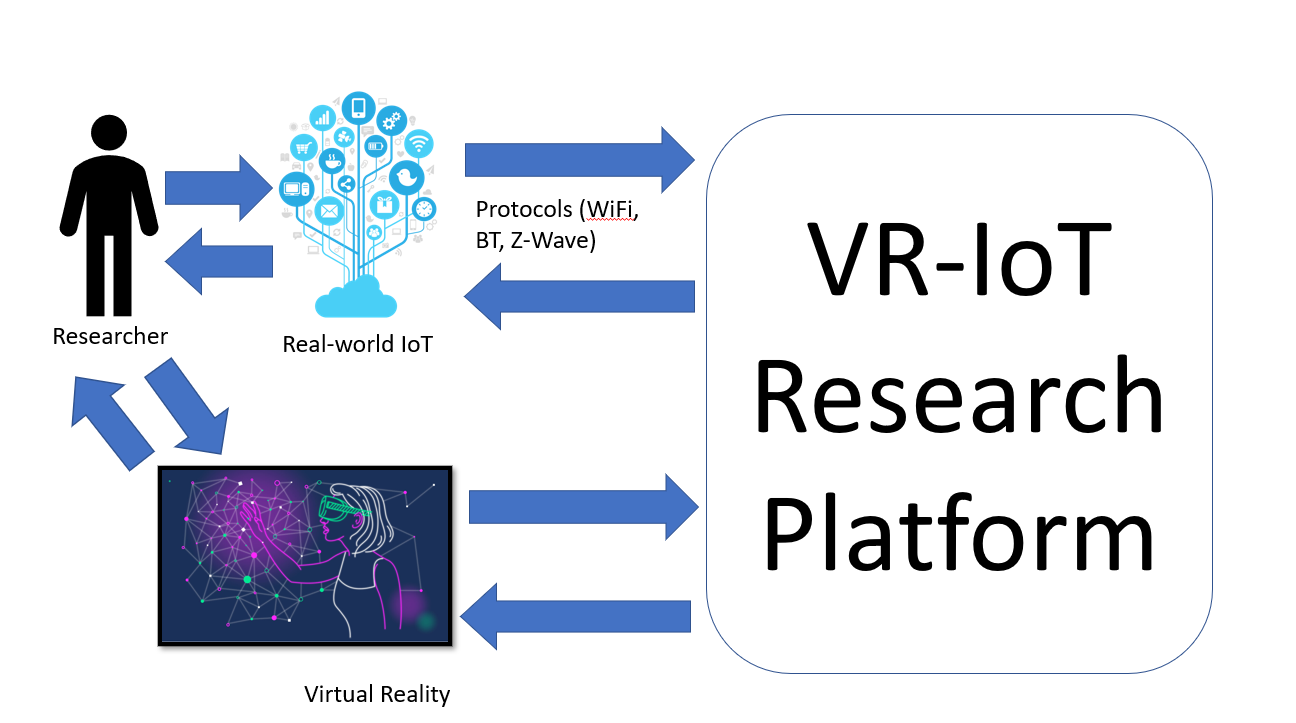
\includegraphics[width=0.9\linewidth]{figures/VR-IoTResearchPlatformLayer.png}
  \caption{VR-IoT Research Platform layer}
  \label{fig:VR-IoTResearchPlatformLayer-figure}
\end{figure}

In Chapter 3, the author proposes a prototype for the platform, with its evaluation in Chapter 4. In Chapter 5, important assumptions are made on how the platform should be designed in terms of architecture and API to connect to the real-virtual world IoT devices. The development cycle and the previous prototypes are discussed in Chapter 6. The platform usage examples in the existing projects are given in Chapter 7. Chapter 8 includes future directions and the conclusion.

Summarizing the problem definition and research idea:

\begin{itemize}
    \item Problem definition: There is no instrument for fast creating, testing, and integrating new IoT devices inside an existing real-world environment.  
    \item Research idea: Define a layer between real-world IoT devices and Virtual Reality. Create a prototype, evaluate the performance and usability and summarize the outputs to explain why the selected architecture can be used as the basis for the future product used to design new IoT devices.
\end{itemize}
% !TeX root = ../thuthesis-example.tex

% Input your chapter title here
\chapter{LITERATURE REVIEW}


The literature review incorporates three sections: research on building an IoT platform without required support of VR, research on interacting with IoT devices in VR and AR, and, at last, research on creating an IoT-VR Platform.

\section{Managing IoT}

Even though using IoT is already considered profitable by many businesses, and automated control saves 
time and money for companies, the problem of connection between heterogeneous IoT devices has not been solved yet. The frameworks existing nowadays which try to solve this issue seem to be usually not user-friendly and not easy-to-use. 

The providers of services of IoT integration into businesses state that using their solutions a big 
amount of data from the connected IoT devices can be analyzed and then turned into actionable 
insights (TODO: add to references https://www.softwareag.com). The insights can be used for lowering energy consumption, analyzing the sensors data etc. These insights can be integrated into the VR-IoT Research platform.

The limitations of the solutions for businesses are:
\begin{enumerate}
    \item Price
    \item No access to the source code
\end{enumerate}

Even if researchers and companies, who are going to be the users of the VR-IoT platform can afford paying high price for getting the analyzed data, they still will not have access to the source code, as well as access to the data used for training the models. Users will need to pay for the subscription to the services, and it will require additional time and money to switch to another solution.

In \cite{k_mohapatra_solution_2016} it is discussed how the framework for connecting heterogeneous devices should operate the incoming data. In this paper the requirements for managing IoT are given: the communication protocols, security and access control and how the data should be analyzed. In section 4 a Reference IoT-Architecture model is proposed. Each of the solution blocks, such as Data Lake or Event Broker is briefly introduced, but since neither implementation nor tests are given, it can not be considered a good structure.

The IoT Architectural Framework, proposed in \cite{uviase_iot_2018}, is based on the Service Oriented Architecture (SOA). This paradigm is used to minimize system integration problems, but when the number of services increases, the performance of the solution can drop. In this article a minimum measures for IoT framework to make the integration easier are proposed \footnote{These measures are used in the requirements for building a VR-IoT platform prototype, described in chapter 3 of this research.} Authors introduce several existing IoT frameworks following the SOA paradigm, and propose their own approach. As it is stated in the paper, the framework has not been implemented, but helps IoT community to understand, in which direction to solve the integration problem.

Compared to \cite{k_mohapatra_solution_2016}, in \cite{ahmad_software_2021} authors provide deeper explanation of how to create an Internet Of Things Driven Data Analysis by using evidence-based software engineering approach. In the article 17 academic publications and industrial solution processes are listed. The authors have created a criteria-based framework, by evaluating different activities for the listed 17 IoT-DA applications and giving an evaluation score for each of the solutions. In the result, each of the applications listed can be used in a specific domain, such as Disaster Management or Environmental Monitoring, but none of them has been associated with a domain of a research for IoT. Even though each of the listed criteria fulfilment was satisfactory at least for one solution, none of the solutions could be considered universal, but can be integrated into other solutions, as well as in VR-IoT Research Platform.

In chapter 1 it was mentioned how creating of 6G can influence the IoT market. In \cite{guo_enabling_2021} a comprehensive study was done, with explanation of how 5G limitations for massive IoT can be overcome by using 6G networks. It was explained how machine learning and blockchain can play the main role in IoT ecosystems. New technologies can be supported such as holographic communications, which can be easily tested in VR-IoT Research Platform.

\section{Interacting with IoT devices in VR and AR}

Augmented reality is used to overlay digital objects onto the objects surrounding us in real life. Extra virtual elements can be attached to the real-world devices. The main idea of the research articles mentioned further is to create a two-way synchronization between Augmented reality and real world: changes in the virtual world are applied to the real world and vice-versa.

Rendering digital devices for Augmented reality and Virtual reality is different: in augmented reality it is impossible to replace the real element with a virtual one. Creating Virtual reality environment similar to the real-world environment requires more time and effort compared to scanning objects to use them in Augmented reality, but in result researchers can have more freedom, such as changing any object parameters. 
In \cite{ankireddy_augmented_2019} authors developed image processing-based approach to control a specific device in real-world by pointing on it with their phone camera and pressing the button (turn the fan On and Off). Their solution is simple but at the same time it shows that it is possible to control IoT devices inside AR at a very low cost. Similar results were achieved in \cite{jo_-situ_2016}, where a generic AR framework for managing IoT devices was proposed, and in \cite{alam_augmented_2017} for creating a safety system by viewing monitoring information on a AR device screen when pointing at the object.

One of the most popular Mixed reality headsets is Microsoft Hololens. Using this device, it is possible to use hands recognition, as well as use API for spatial awareness. In \cite{sun_magichand_2019} authors proposed used deep learning approach to create a tool for interacting with IoT devices using hand gestures. 
Cities such as Shanghai, New York, Moscow can already be considered as smart cities, because they have been implementing smart solutions for several years already. Using Augmented and Virtual reality can help in creating IoT solutions for such smart cities and networks, as it is shown in \cite{chakareski_uav-iot_2019}, \cite{carneiro_bim_2018}. As for other domains, in \cite{paul_role_2019} it was shown how AR and VR combined with IoT can be used for smart education, and in \cite{jang_building_2019-1} for energy management. In sum, using AR and VR for managing IoT has been proved to be effective.

\section{IoT-VR platforms}

The research has no novelty, if a solution already exists. Fortunately, none of the following articles is focused on creating a platform for creating new IoT devices using VR.

Nonetheless, the following articles are helpful for developing VR-IoT platform.

In the previous section it was explained how 6G can influence the IoT market. In \cite{liao_information-centric_2021} authors provide their solution for integrating AR/VR inside 6G massive IoT environment.

As mentioned above, using VR for IoT research requires building a virtual environment. Nowadays most of VR headsets provide 6 degrees of freedom, which means that it can be possible to move in the real world and virtual world at the same time. In \cite{you_internet_2018} authors research how IoT can be used for seamless virtual reality space created by 360 degree photos and videos.

In \cite{myeong-in_choi_design_2017}, \cite{simiscuka_synchronisation_2018}, \cite{simiscuka_real-virtual_2019}, \cite{krishnan_performance_2020} VR-IoT platforms were proposed, but none of the articles is focused on implementing a universal solution, which can be used for research in IoT. Instead, only demos for particular devices are provided, and overall the research can not be considered deep enough by the author.

Finally, in \cite{hu_virtual_2021} a research on VR headsets market was provided, and several applications of VR in IoT were proposed. The authors mainly focused on VR streaming solutions.

Overall, many examples of using VR for IoT have been proposed in the literature, and can be summarized into following insights:
\begin{enumerate}
    \item 6G networks will enable using new types of IoT devices, based on deep learning and blockchain, and it will make possible to send huge amount of data for seamless VR experience;
    \item AR can enrich operation with real-world IoT devices by layering extra data on top of them;
    \item The latency of VR-IoT experience is small enough to provide good user experience.
\end{enumerate}

In the next chapter the VR-IoT platform requirements are defined, as well as the prototype is introduced.
% !TeX root = ../thuthesis-example.tex

\chapter{PROTOTYPE OF VR-IoT Research Platform}

\section{Platform requirements}
Firstly, we define the requirements our platform should follow:
\begin{enumerate}
\item Scalability. The performance of the platform should stay acceptable when the number of devices in our system increase;
\item Ease of use and testing. Since using Virtual Reality and IoT devices requires interacting with different kinds of elements, we need to provide a natural way of interacting with such objects. As for real-world devices we only need to implement sensor data collection, creating an API for virtual reality digital representation of such devices can be a challenge. Another important task is simulation of VR interactions on a computer for ease of testing;
\item Fault Tolerance. As if we are not developing the IoT devices themselves, platform should effectively handle faults coming from both sides (real and virtual worlds);
\item Simultaneous work. As in the real world, when several people can interact with an IoT system, each of the running instances of the platform should be able to run simultaneously and operate with the same data.
\end{enumerate}
The architecture of the platform has to be based on three layers, which we further modify and extend with extra connections: 
\begin{enumerate}
    \item Real-world IoT devices HUB. In order to collect the data from real-world devices, we need a special device responsible for receiving and sending the data to them. In commercial market, usually mobile phone apps have interface to interact with IoT devices (Mi Home APP, HomeKit App etc), but since we require using the data in virtual reality (which is a different interface), we need to operate with IoT sensors data on a special HUB, which can provide the data in a unified format (abstraction of sensors)
    \item Integration layer. This is the main part of the platform. Analyzing data coming from VR and from real world, integrating real-world devices data into VR and vice-versa, performing persistence and providing API for using the platform in research projects;
    \item Visualization layer. Interaction with digital IoT devices can be performed using VR headsets, AR devices or by simulating the touch, sight, gestures and other interactions. Our aim is to provide an API for developers to integrate their interaction techniques into this layer, but developing these techniques is not the focus of this research. 
\end{enumerate}

\section{Real-world IoT devices HUB}
To support different IoT devices in out platform, either a standalone or third-party software can be used. By analyzing the market, we have agreed on using a third-party software openHAB with a future upgrade to our own solution. The Hub we use runs on a server and is responsible for collecting and storing the data coming from IoT devices. Managing the data is performed through a web interface, while API is based on REST calls.

\section{Integration layer}
By receiving and sending unified data objects representing IoT devices sensor data using REST API calls, each of the running instances of the NUIX-Studio App (our platform) running in the Integration layer will operate with the same data, enabling simultaneous work.
Next step is to represent IoT devices data in virtual reality and perform computations for research. Since the platform should run smoothly on VR headsets and provide good UX, the computations should be performed on a high-performance PC, while interaction with virtual IoT devices is done by using VR headsets. 

\section{Visualization layer}
Since the platform purpose is to provide an API for research on IoT devices in VR, we decided to use Unity for interaction with virtual reality devices. First of all, by choosing Unity, we save time from developing our own 3D engine. Secondly, we can build the project for most of platforms and provide support for VR headsets. And thirdly, developers are already familiar with Unity development, and can integrate their research projects into the platform faster than if we used our own 3D engine.

This is an example of an appendix image: (Figure~\ref{fig:BasicPlatformStructure-figure})

\begin{figure}
  \centering
  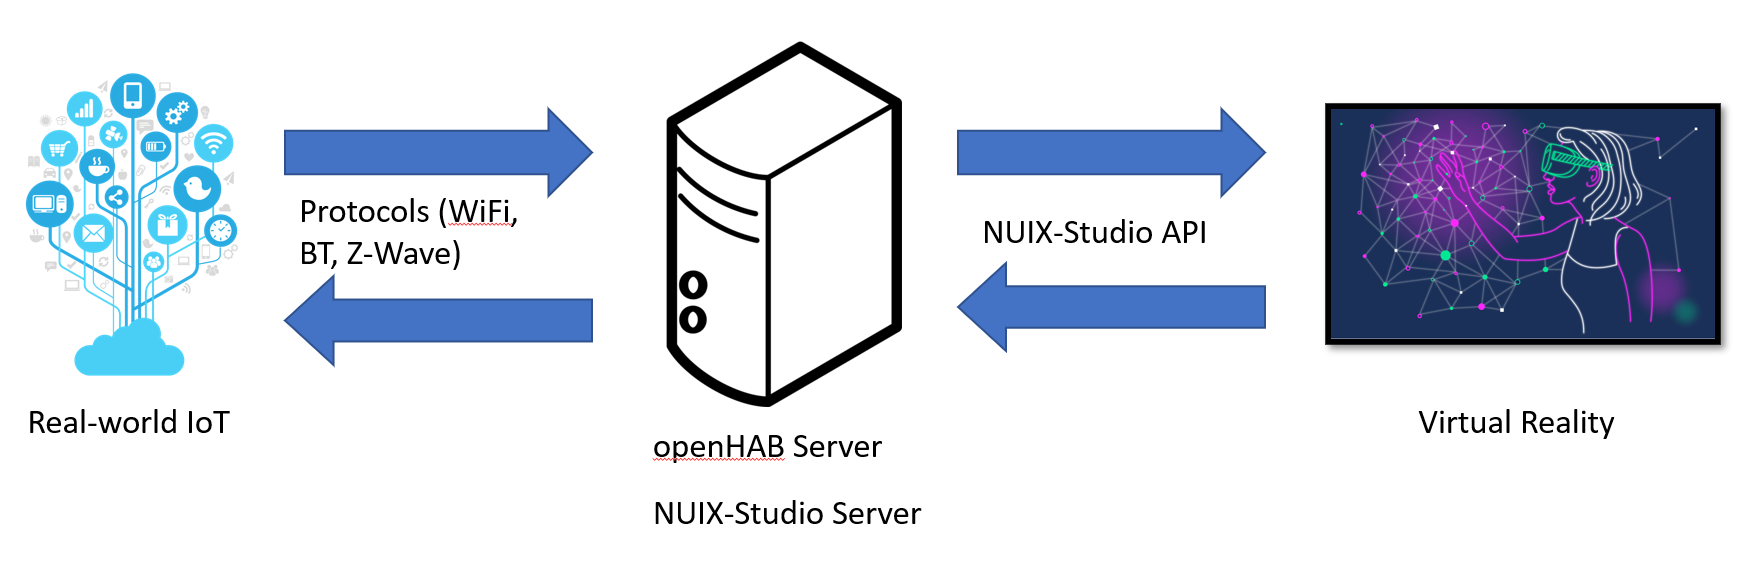
\includegraphics[width=0.6\linewidth]{figures/BasicPlatformStructure.png}
  \caption{Simplified structure of NUIX Studio. Real-world IoT devices HUB is openHAB server, while NUIX-Studio server is the main instance of NUIX-Studio APP responsible for the computations.}
  \label{fig:BasicPlatformStructure-figure}
\end{figure}

\section{Server Architecture}
\subsection{OpenHAB Server Structure}

Before we explain the structure of our server, we first give definitions for the base elements of openHAB:

Things are entities that can be physically added to a system. Things may provide more than one function (for example, a Z-Wave multi-sensor may provide a motion detector and also measure room temperature). Things do not have to be physical devices; they can also represent a web service or any other manageable source of information and functionality.

Things expose their capabilities through Channels. Whether an installation takes advantage of a particular capability reflected by a Channel depends on whether it has been configured to do so. When you configure your system, you do not necessarily have to use every capability offered by a Thing. You can find out what Channels are available for a Thing by looking at the documentation of the Thing's Binding.

Bindings can be thought of as software adapters, making Things available to your home automation system. They are add-ons that provide a way to link Items to physical devices. They also abstract away the specific communications requirements of that device so that it may be treated more generically by the framework.

Items represent capabilities that can be used by applications, either in user interfaces or in automation logic. Items have a State and they may receive commands.

The glue between Things and Items are Links. A Link is an association between exactly one Channel and one Item. If a Channel is linked to an Item, it is "enabled", which means that the capability the Item represents is accessible through that Channel. Channels may be linked to multiple Items and Items may be linked to multiple Channels.



\section{Symbols}

As required by the national formatting standards, the template uses \pkg{unicode-math} for formatting mathematical symbols, which differs to the default used by LATEX. 

\begin{enumerate}
  \item Capital Greek letters are italic by default e.g. \cs{Delta}:$\Delta$。
  \item Increment symbol: $\increment$(U+2206)
  \item Vectors, matrices, tensors should be ITALIC, and BOLD using the \cs{symbf} command; for example: $\symbf{A}$, $\symbf{\alpha}$.
  \item For constants and special functions, use the \cs{symup} command. For example:
    $\symup{\pi} = 3.14\dots$; $\symup{e} = 2.718\dots$,
  \item Example of integrals and differentials: $\int f(x) \dif x$。
\end{enumerate}

For more usage of symbols, you could use the following references
\href{http://mirrors.ctan.org/macros/latex/contrib/unicode-math/unicode-math.pdf}{\pkg{unicode-math}}
\href{http://mirrors.ctan.org/macros/latex/contrib/unicode-math/unimath-symbols.pdf}{\pkg{unimath-symbols}}.

For units and metrics, it is recommended to use the following package:
\href{http://mirrors.ctan.org/macros/latex/contrib/siunitx/siunitx.pdf}{\pkg{siunitx}}
It can conveniently handle the space between Greek letters/numbers and the unit. For example:
\SI{6.4e6}{m},
\SI{9}{\micro\meter},
\si{kg.m.s^{-1}},
\SIrange{10}{20}{\degreeCelsius}。



\section{Mathematical formula}

You can use the following environments \env{equation} 和 \env{equation*} for mathematical formulae.

Please pay attention that round brackets should be included before and after referencing an equation: e.g. Equation \eqref{eq:example}.

\begin{equation}
  \frac{1}{2 \symup{\pi} \symup{i}} \int_\gamma f = \sum_{k=1}^m n(\gamma; a_k) \mathscr{R}(f; a_k)
  \label{eq:example}
\end{equation}

When there are multiple equations, please try to align them at the "equal" sign if possible. We recommend using the \env{align} environment.
For example:
\begin{align}
  a & = b + c + d + e \\
    & = f + g
\end{align}


\section{Mathematical axioms and proofs}

You can use \pkg{amsthm} or \pkg{ntheorem} packages to set up your axiom. After loading one of those package, the template will automatically setup the environments: \env{theorem} and \env{proof}

An example:
\begin{theorem}[Lindeberg--Lévy Central Limit Theorem]
  Set random variables $X_1, X_2, \dots, X_n$ i.i.d., with expectation mean of $\mu$ and variance $\sigma^2 \ne 0$. By formula, $\bar{X}_n = \frac{1}{n} \sum_{i+1}^n X_i$, we have
  \begin{equation}
    \lim_{n \to \infty} P \left(\frac{\sqrt{n} \left( \bar{X}_n - \mu \right)}{\sigma} \le z \right) = \Phi(z),
  \end{equation}
  where $\Phi(z)$ is the function of a normal distribution.
\end{theorem}
\begin{proof}
  Trivial.
\end{proof}

The template also provides the following environments: \env{assumption}、\env{definition}、\env{proposition}、
\env{lemma}、\env{theorem}、\env{axiom}、\env{corollary}、\env{exercise}、
\env{example}、\env{remar}、\env{problem}、\env{conjecture} 
% !TeX root = ../thuthesis-example.tex

\chapter{VR-IOT RESEARCH PLATFORM PERFORMANCE TESTING}

In this chapter, one of the most common IoT environments Smart home is used to create a device of a new type. There are several devices in the example configuration (Figure~\ref{fig:TestingEquipment-figure}):
\begin{enumerate}
    \item A Smart Wi-Fi lamp;
    \item A PC running openHAB server and NUIX-Studio App instance;
    \item A PC running NUIX-Studio App instance;
    \item An Oculus Quest VR Headset;
    \item A smart vacuum cleaner.
\end{enumerate}

\begin{figure}
  \centering
  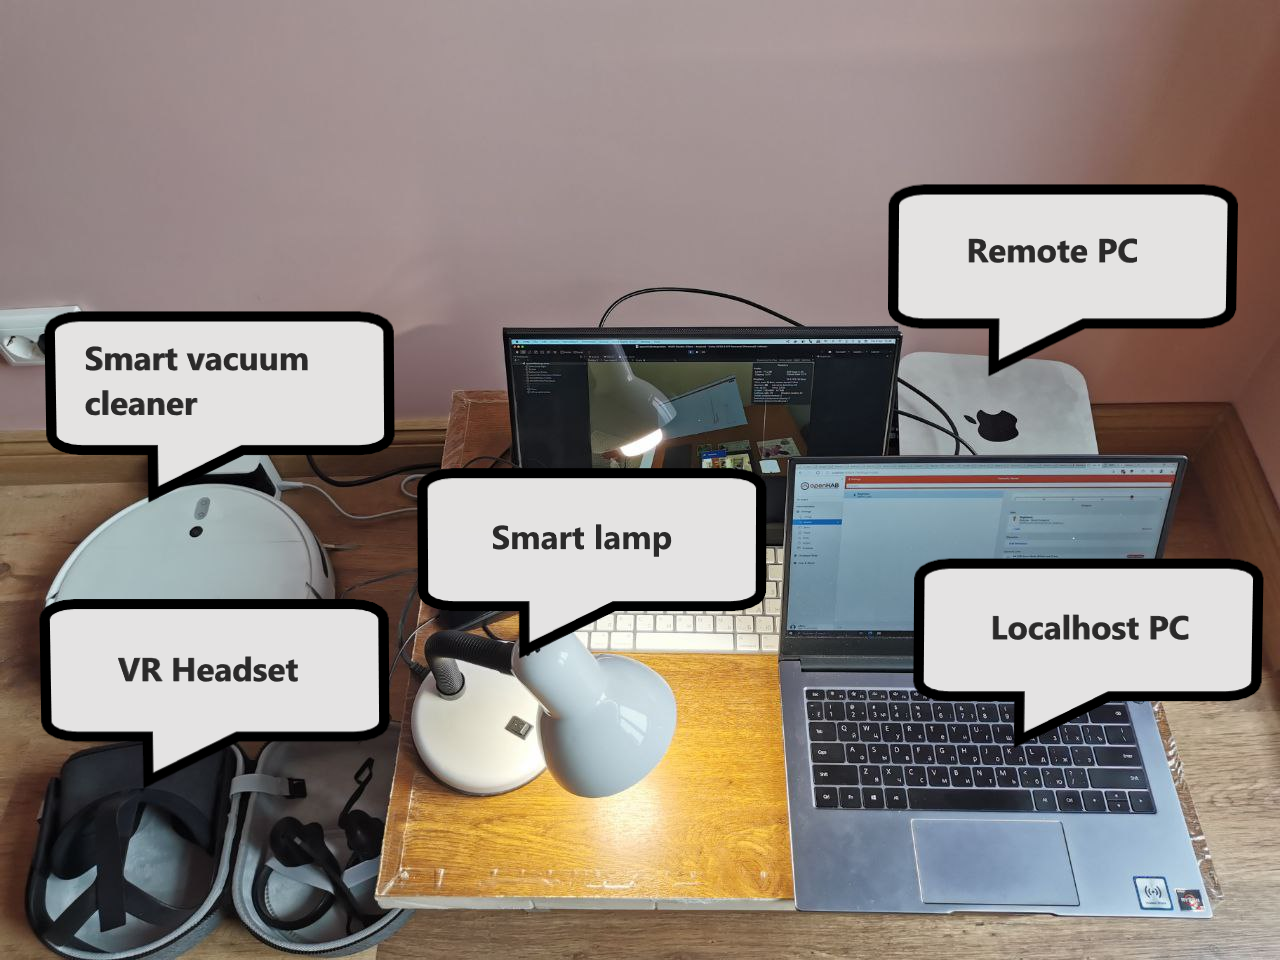
\includegraphics[width = 0.9 \linewidth]{figures/TestingEquipment.png}
  \caption{Testing equipment.}
  \label{fig:TestingEquipment-figure}
\end{figure}

In the following experiments, gesture control functionality is added for the smart lamp\footnote{Smart vacuum cleaner and remote PC will be used in the next experiment}.

Widgets for Light and Gesture Recognition are created in the virtual environment scene. In other words, virtual lamp light is equivalent to the real-world one, and a gesture control interface is implemented.

\section{Server setup}
As a first step, a binding needs to be added to the openHAB server. Xiaomi Mi IO binding makes it possible to automatically add the Xiaomi Smart Wi-Fi Lamp to the server (Figure~\ref{fig:ServerSetupProcedure-figure}).

\begin{figure}
  \centering
  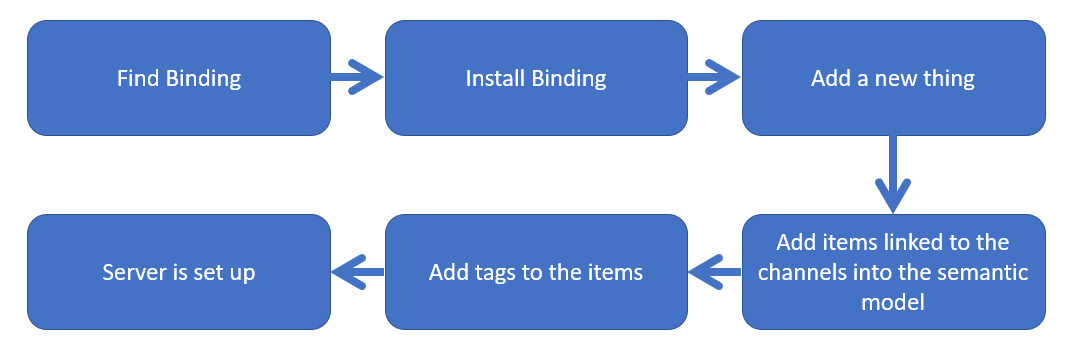
\includegraphics[width = 0.9 \linewidth]{figures/ServerSetupProcedure.png}
  \caption{Server setup procedure.}
  \label{fig:ServerSetupProcedure-figure}
\end{figure}

The next step is adding items linked to the lamp channels. In the example, the lamp brightness dimmer is added to the semantic model. As seen in Figure~\ref{fig:SemanticModelOne-figure}, the user can move the dimmer to control the lamp's light brightness. The real-world lamp will change the brightness based on the value on the server.

\begin{figure}
  \centering
  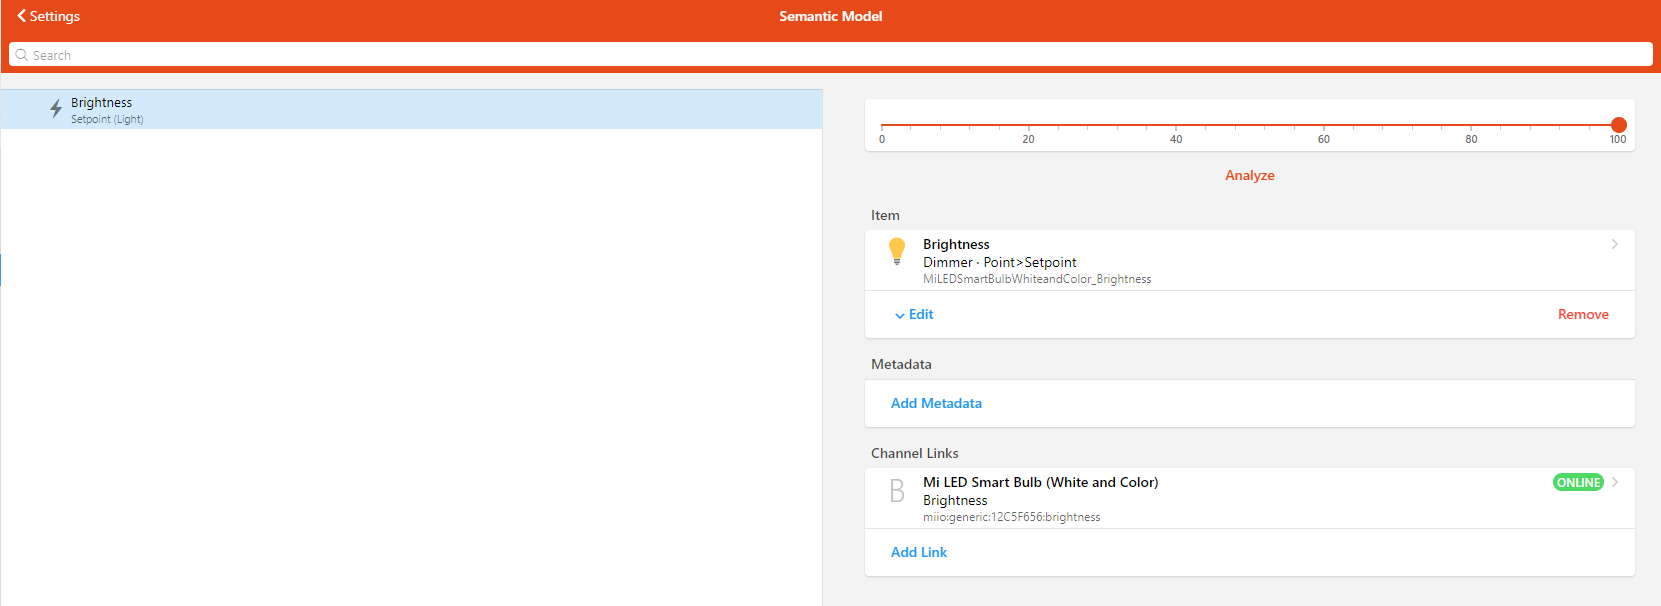
\includegraphics[width = 0.9 \linewidth]{figures/SemanticModelOne.png}
  \caption{Semantic model 1.}
  \label{fig:SemanticModelOne-figure}
\end{figure}

The next step is adding item tags for gesture control and for the light visualization (Figure~\ref{fig:ItemEditPage-figure}).

\begin{figure}
  \centering
  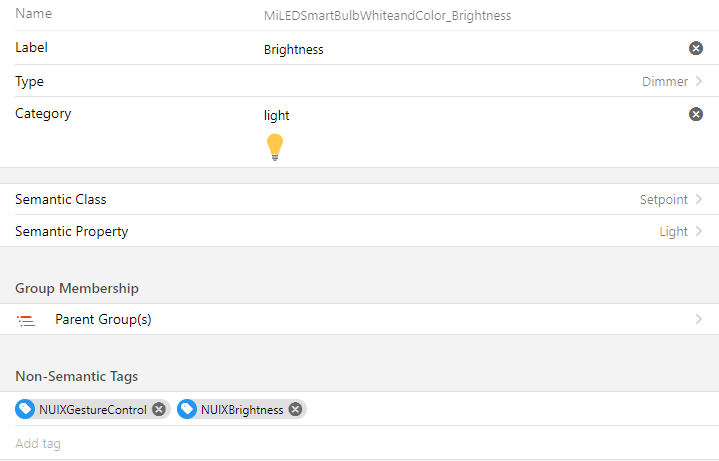
\includegraphics[width = 0.9 \linewidth]{figures/ItemEditPage.png}
  \caption{Item Edit Page.}
  \label{fig:ItemEditPage-figure}
\end{figure}

The server has been set up for connection to NUIX-Studio App instances.

\section{Running NUIX-Studio App}

After the server has been set up and the Smart home environment has been chosen, the platform App instances are ready to run on the devices.

(A screenshot with gesture control).

In the experiment, a VR-IoT platform user performs three actions:
\begin{enumerate}
    \item Put on Virtual reality headset;
    \item Press the virtual button to establish a Client-Server connection and receive the items list;
    \item Perform a "Thumb up" gesture. By rotating the fist, the lamp brightness changes in the VR-IoT environment \footnote{Both in real and virtual worlds}.
\end{enumerate}

The user of the platform performed these actions\footnote{In this experiment, the platform developer performed the user role.}. Thus, support for gestures was added to control the lamp's brightness, and the experiment to create a new device for the existing environment can be considered a success.

\section{Performance analysis}

The analysis of platform performance is not the study's primary goal, but it helps to find bottlenecks. 

The following experiment shows that it is viable to perform rendering tasks on a separate server. Having a common database for all instances of the application will help achieve several users' simultaneous work within the system.

The first experiment is the system startup analysis, performed on three devices by registering the startup time (Figure~\ref{fig:SystemStartupScheme-figure}).

\begin{figure}
  \centering
  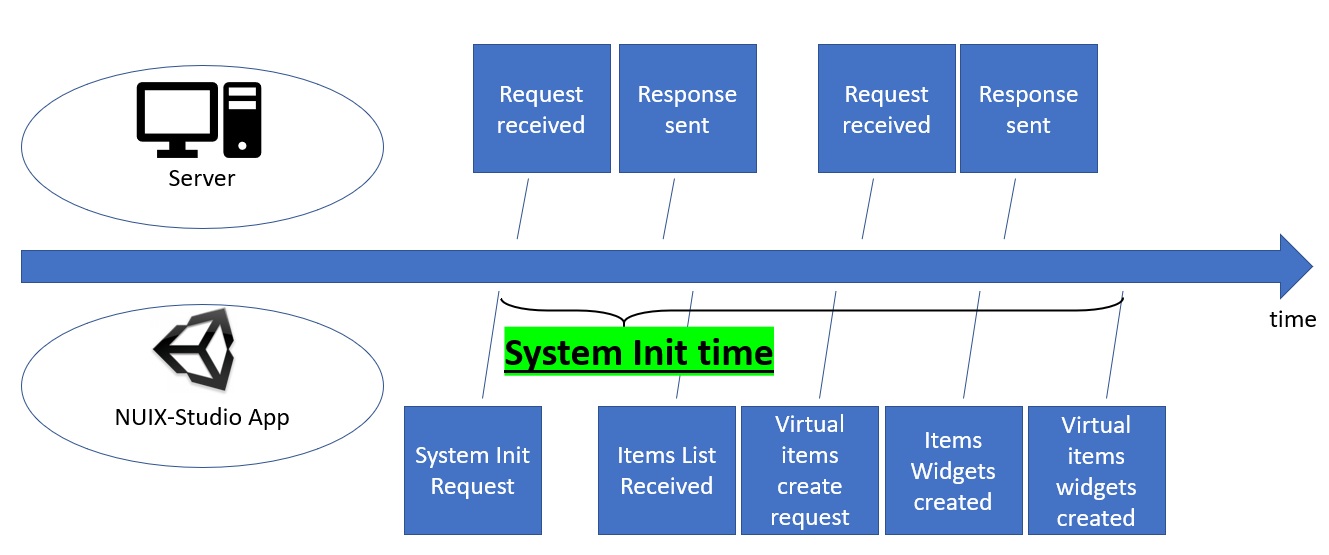
\includegraphics[width = 0.9 \linewidth]{figures/SystemStartupScheme.png}
  \caption{System startup scheme.}
  \label{fig:SystemStartupScheme-figure}
\end{figure}

The hardware specifications are listed in Table~\ref{tab:hardware-specifications-table} \footnote{Localhost PC is a notebook running openHAB server as well as one instance of NUIX-Studio APP; Remote PC is a computer running one instance of NUIX-Studio APP and connected to the same Wi-Fi network as localhost PC; Oculus Quest is a Virtual Reality Headset running NUIX-Studio APP and connected to the same Wi-Fi network as PCs.}.

\begin{table}
  \centering
  \begin{threeparttable}[c]
    \caption{Hardware specifications in the experimental setup}
    \label{tab:hardware-specifications-table}
    \begin{tabular}{ll}
      \toprule
      Unit    &         Specifications                 \\
      \midrule
      Localhost PC & Ryzen 5 3500u, Windows 10 \\
      Remote PC & Core i5 4278U, macOS 11.2.3    \\
      Oculus Quest        & Qualcomm Snapdragon 835, Android-based            \\
      \bottomrule
    \end{tabular}
  \end{threeparttable}
\end{table}

Each test was performed on a new Unity APP instance to avoid cashing influence. And then mean values have been calculated (Figure~\ref{fig:SystemInitTime-figure}).

\begin{figure}
  \centering
  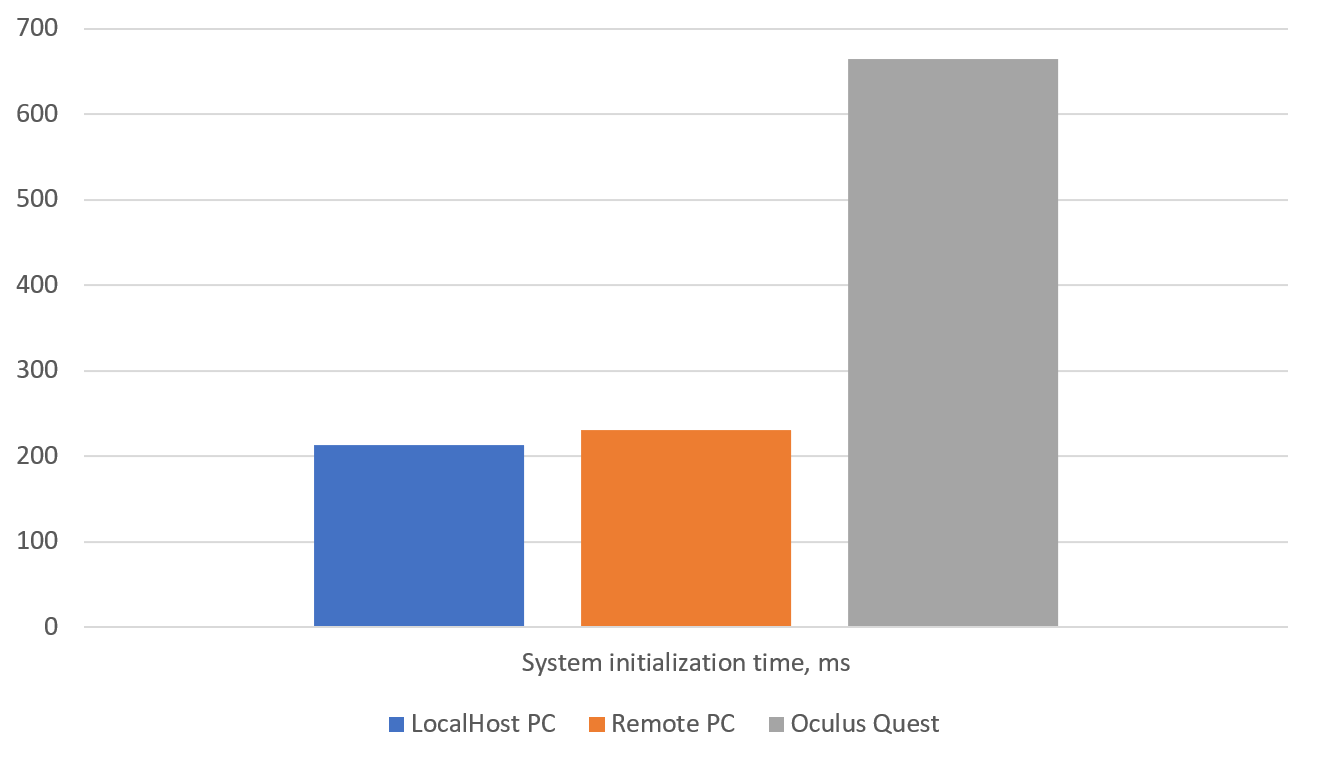
\includegraphics[width=0.9\linewidth]{figures/SystemInitTime.png}
  \caption{System initialization time measured on different client devices, in ms}
  \label{fig:SystemInitTime-figure}
\end{figure}

As seen in Figure~\ref{fig:SystemInitTime-figure}, the system initialization time is a time-consuming operation, which takes from 200ms to over 600ms on average to perform.

In the next experiment, event processing time was measured. On one of the devices running the NUIX-Studio App instance, a user changed an Item value \footnote{In this case, the brightness of the smart bulb changed by moving the corresponding pinch slider widget}. The server processed the received request to change the Item parameter, and then an Event containing information about the new Item value was sent to all devices connected to the server. The device on which this Item change occurred ignored the new incoming value because it was equal to the old value. Next, the processing time of a request on another device was measured (Figure~\ref{fig:EventProcessingScheme-figure}).

\begin{figure}
  \centering
  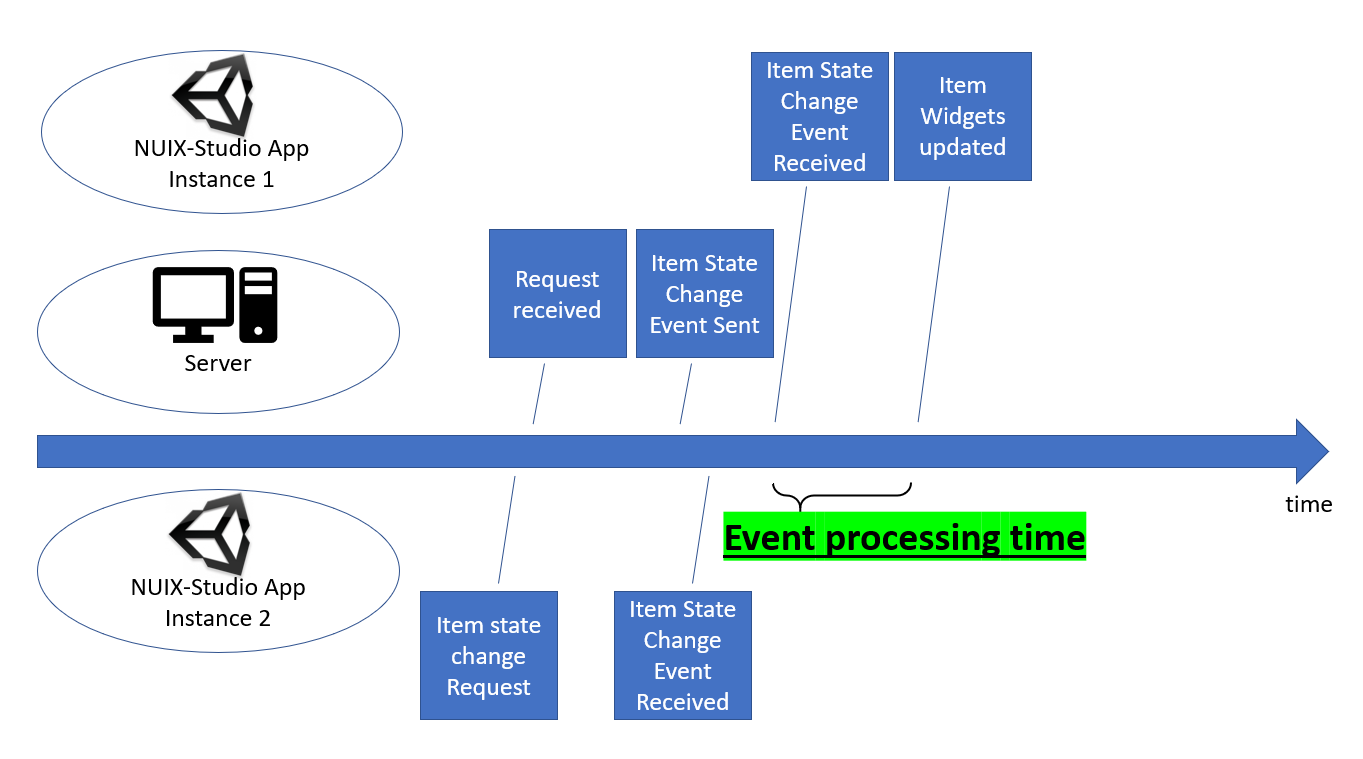
\includegraphics[width = 0.9 \linewidth]{figures/EventProcessingScheme.png}
  \caption{Event processing scheme.}
  \label{fig:EventProcessingScheme-figure}
\end{figure}

As seen on the resulting histogram (Figure~\ref{fig:EventProcessingTime-figure}), Oculus Quest's performance on this test is outstanding. The processing time difference is explained by the fact that the NUIX-Studio App runs in an unoptimized state on Windows and macOS\footnote{Unity editor mode}, but can run significantly faster after the App instances are built for the platforms.

\begin{figure}
  \centering
  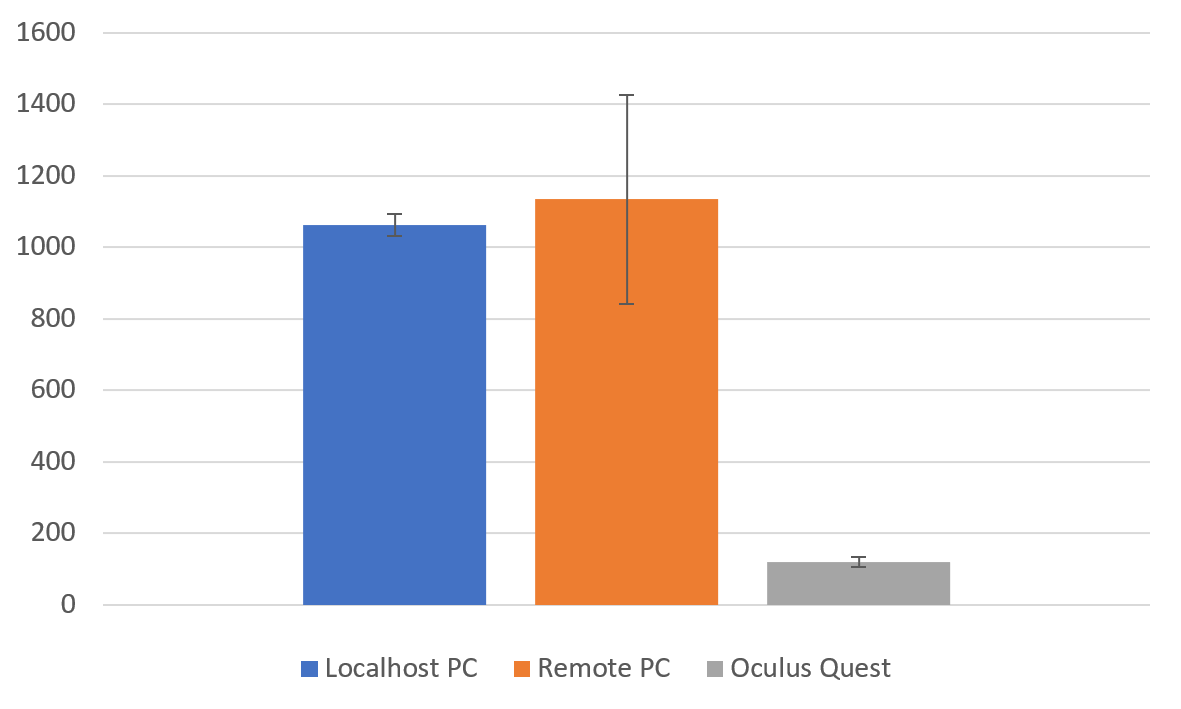
\includegraphics[width = 0.9 \linewidth]{figures/EventProcessingTime.png}
  \caption{Event processing time measured on different devices, in \textmu{}s}
  \label{fig:EventProcessingTime-figure}
\end{figure}

The results of this experiment will be used in the future: system initialization time is long is based on the device hardware performance, and in some later experiments, it is better not to perform time calculations that include system initialization, while event processing time is relatively low, and in most cases, it can be ignored.

The following experiment uses a virtual reality headset, a smart light bulb, and a server running an application on it. For instance, a light sensor is used inside a Smart home environment, located at a relatively large distance from the lamp (2-3 meters), and is triggered when the amount of light falling on its sensor exceeds a certain threshold. For example, this setup is used in industries to provide a comfortable lighting level while keeping an optimal amount of energy consumption. The light sensor triggers precisely at some sufficiently large value of the lamp brightness. Hence, the most accurate adjustment of the brightness level of the light bulb is needed.

The previous experiment showed that gesture control could be used to control a lamp's brightness level. This experiment shows that the transfer of computations from the Virtual reality headset to the server is necessary in a specific case. The user is asked to perform the same steps as in the previous experiment, with one more step added:  setting the brightness to the specified level. Supposing that the light sensor is triggered at a lamp light brightness level of 50 out of 100 \footnote{Using Fitts' law, it can be assumed that setting up brightness levels to different values takes different time. However, this effect is considered not significant for the experiment.}. The user's task is to set the light brightness to the specified value as quickly as possible using gesture control. In order to omit additional operations not related to the direct use of gestures to change the brightness of the lamp, such as starting the system, the user had to repeat the step by setting the brightness of the light to the specified value two times. The interval between the first and second times, when the lamp brightness is equal to the specified value, can be divided into two components (Equation \eqref{eq:totaltime}): the user reaction time to a successful change in the brightness level $ t_{react} $, and the execution time of the new calibrations $ t_{cal} $.


\begin{equation}
  t = t_{react} + t_{cal}
  \label{eq:totaltime}
\end{equation}

Two people participated in the two series of the experiment. In the first series, the light's illumination was computed on a Virtual reality headset, and in the second, on a server that was periodically calculating the light map. User reaction time $ t_{react} $ is a value independent of the changed synchronization parameters. Therefore, the difference in calculated time in the first and the second series of the experiment is equal to the difference in time spent on calibrating the lamp brightness in said experiment (Equation \eqref{eq:deltatime}).

\begin{equation}
  t _{\Delta} = (t_{react} + t_{cal_1}) - (t_{react} + t_{cal_1}) = t_{cal_1} - t_{cal_2}
  \label{eq:deltatime}
\end{equation}

As it can be seen in the Figure~\ref{fig:ExperimentTime-figure}, the time it took the participants to perform the task is unstable, but it is still can be seen that on average it took more time to perform the task in the first series than in the second series for both users. In Figure~\ref{fig:DeltaTime-figure} it can be seen that $t_{\Delta}$ is more than zero for the most observations.

\begin{figure}
  \centering
  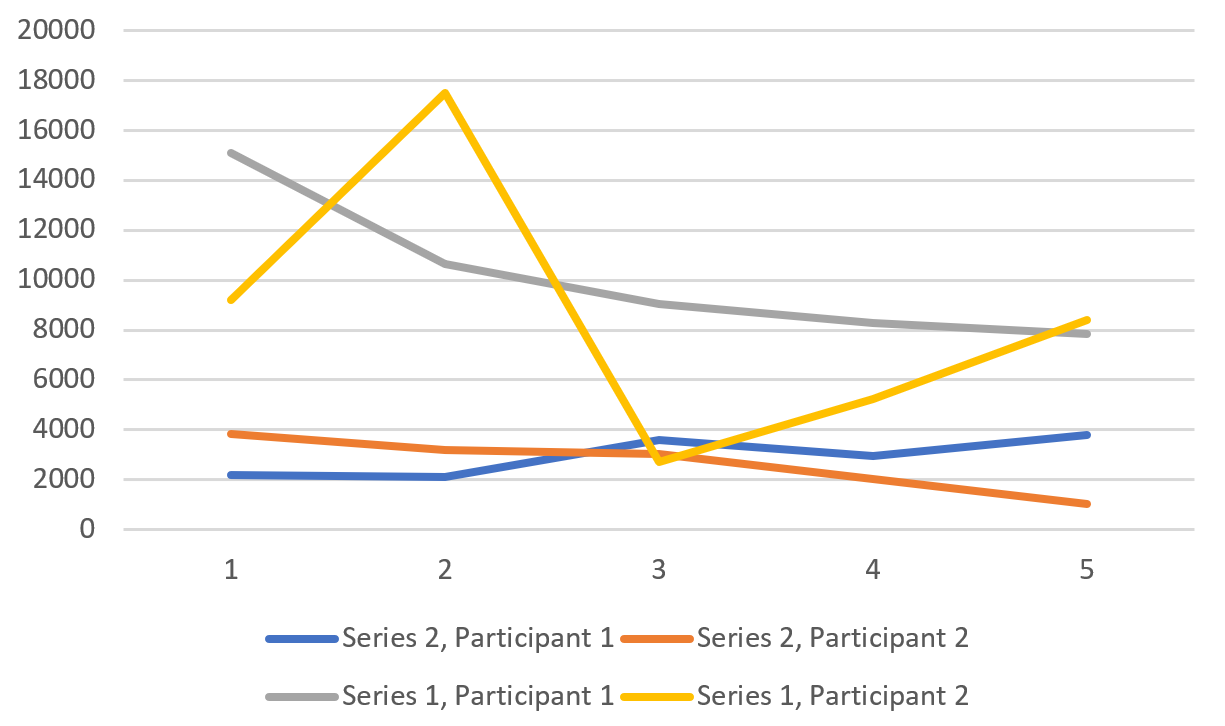
\includegraphics[width = 0.9 \linewidth]{figures/ExperimentTime.png}
  \caption{Time spent on calibrating the lamp brightness, in ms}
  \label{fig:ExperimentTime-figure}
\end{figure}


\begin{figure}
  \centering
  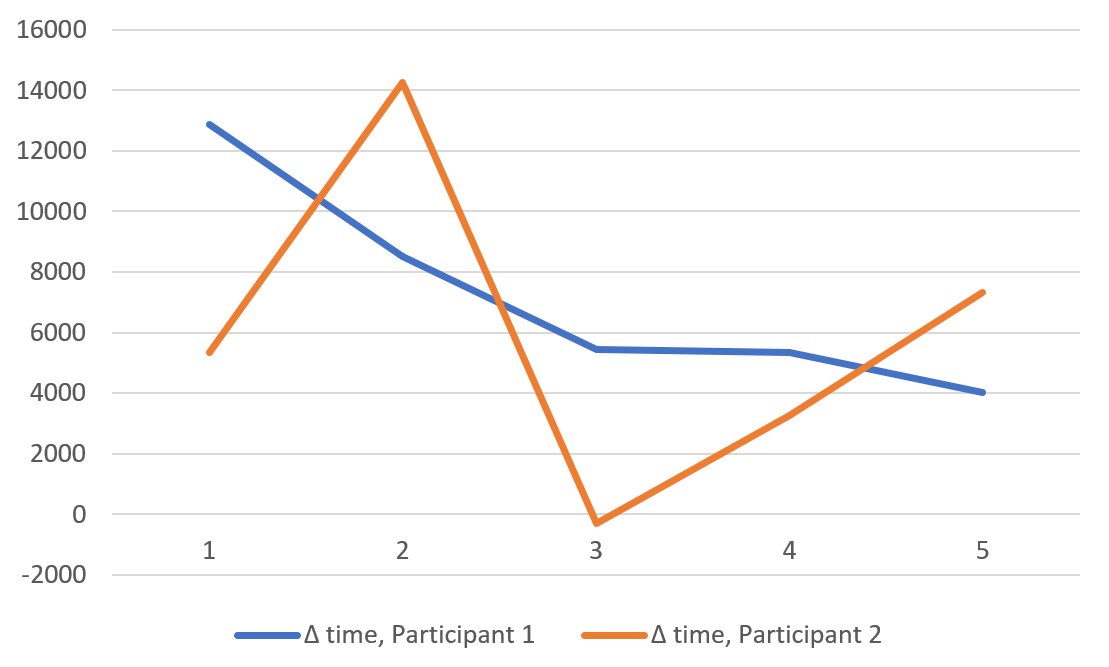
\includegraphics[width = 0.9 \linewidth]{figures/DeltaTime.png}
  \caption{The difference between the time spent on calibrating the lamp brightness in the first and the second series of the experiment, in ms}
  \label{fig:DeltaTime-figure}
\end{figure}

Additional data were also analyzed during the experiment, such as the number of frames per second with which the NUIX-Studio App was rendered on the screen (Figure~\ref{fig:exp-screenshot}). Figure~\ref{fig:Series2FPSpng-figure} shows that in the first series of the experiment, the number of frames per second drops significantly as soon as the system is initialized and widgets for items from the Semantic model are created. In the second series of the experiment, such a drop is no longer observed (Figure~\ref{fig:Series1FPSpng-figure}): because the illumination was computed on a separate device, the number of frames per second drops only slightly \footnote{Probably, because illumination computation is significant for the device's performance, especially its Graphics processing unit.}.

\begin{figure}
  \centering
  \subcaptionbox{Series 1\label{fig:exp-screenshot-a}}
    {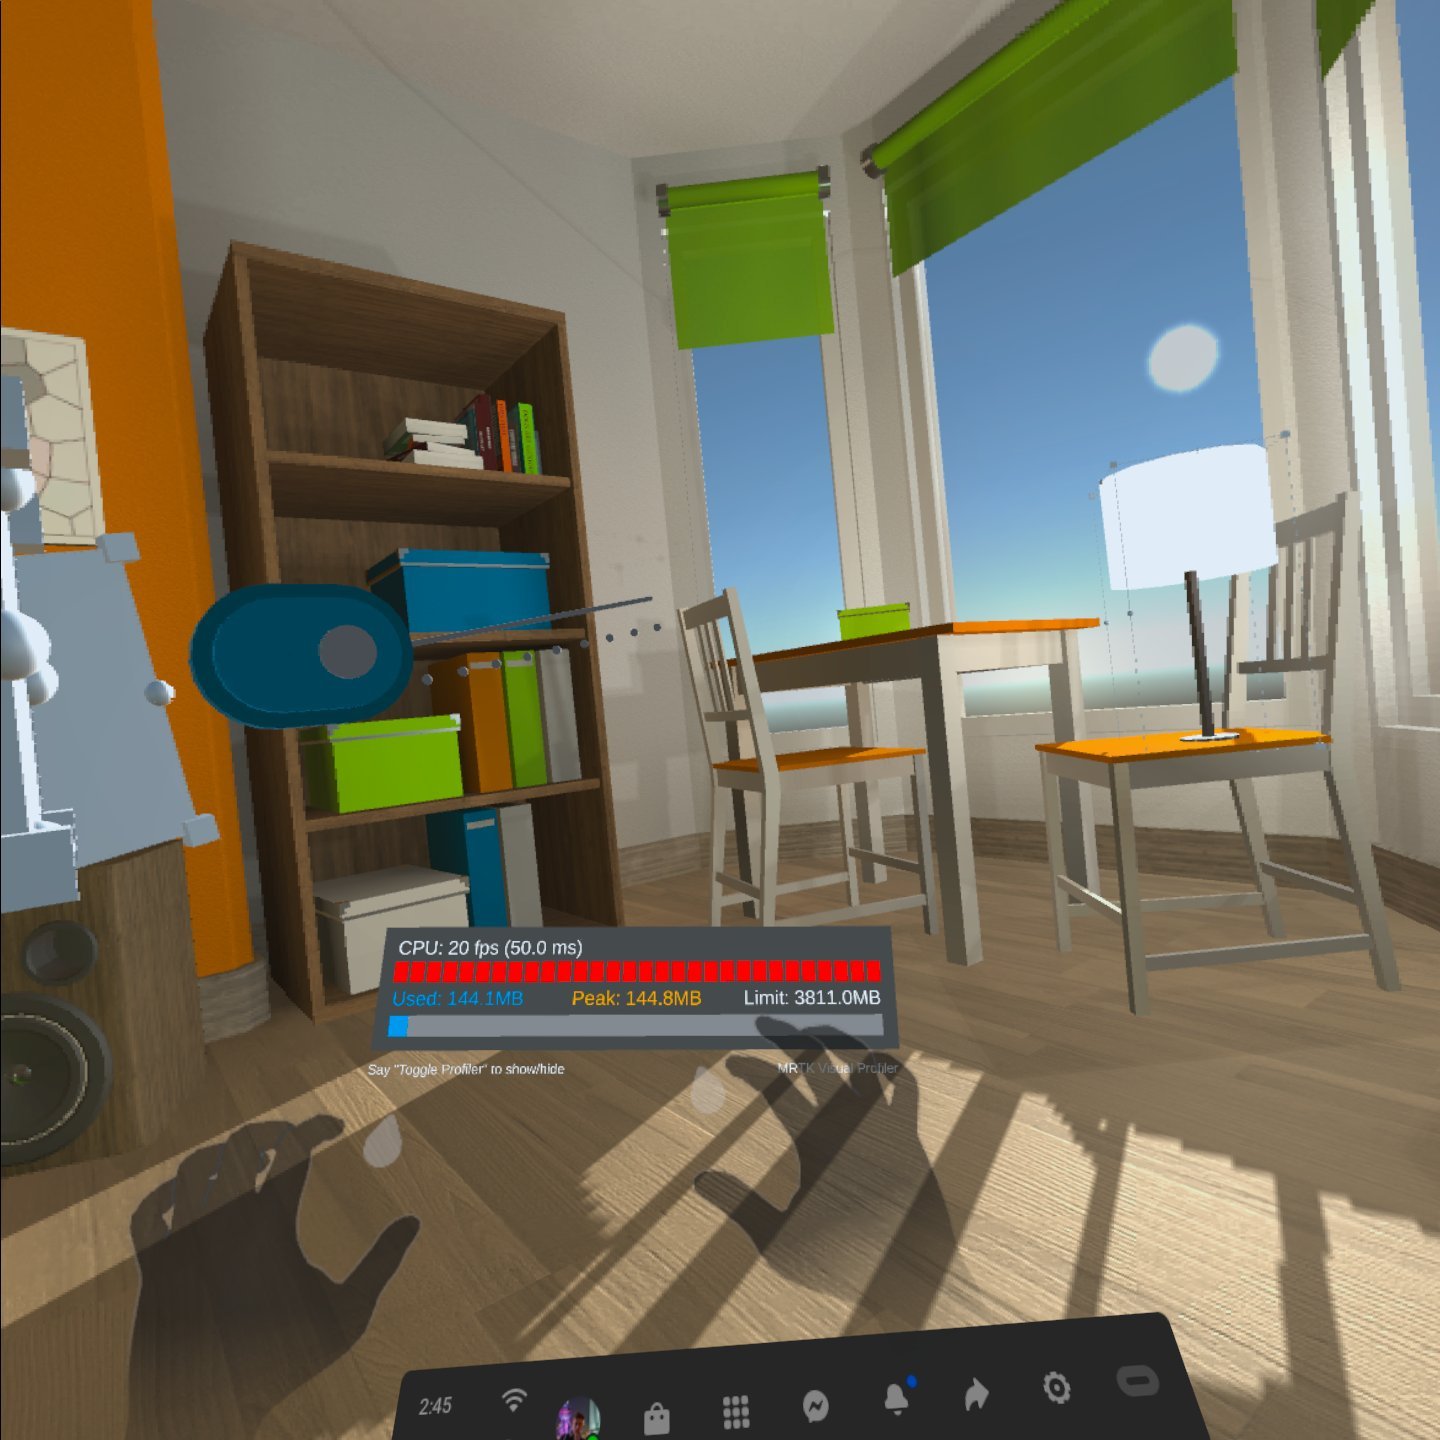
\includegraphics[width=0.45\linewidth]{figures/Series1FPSOculus.jpg}}
  \subcaptionbox{Series 2\label{fig:exp-screenshot-b}}
    {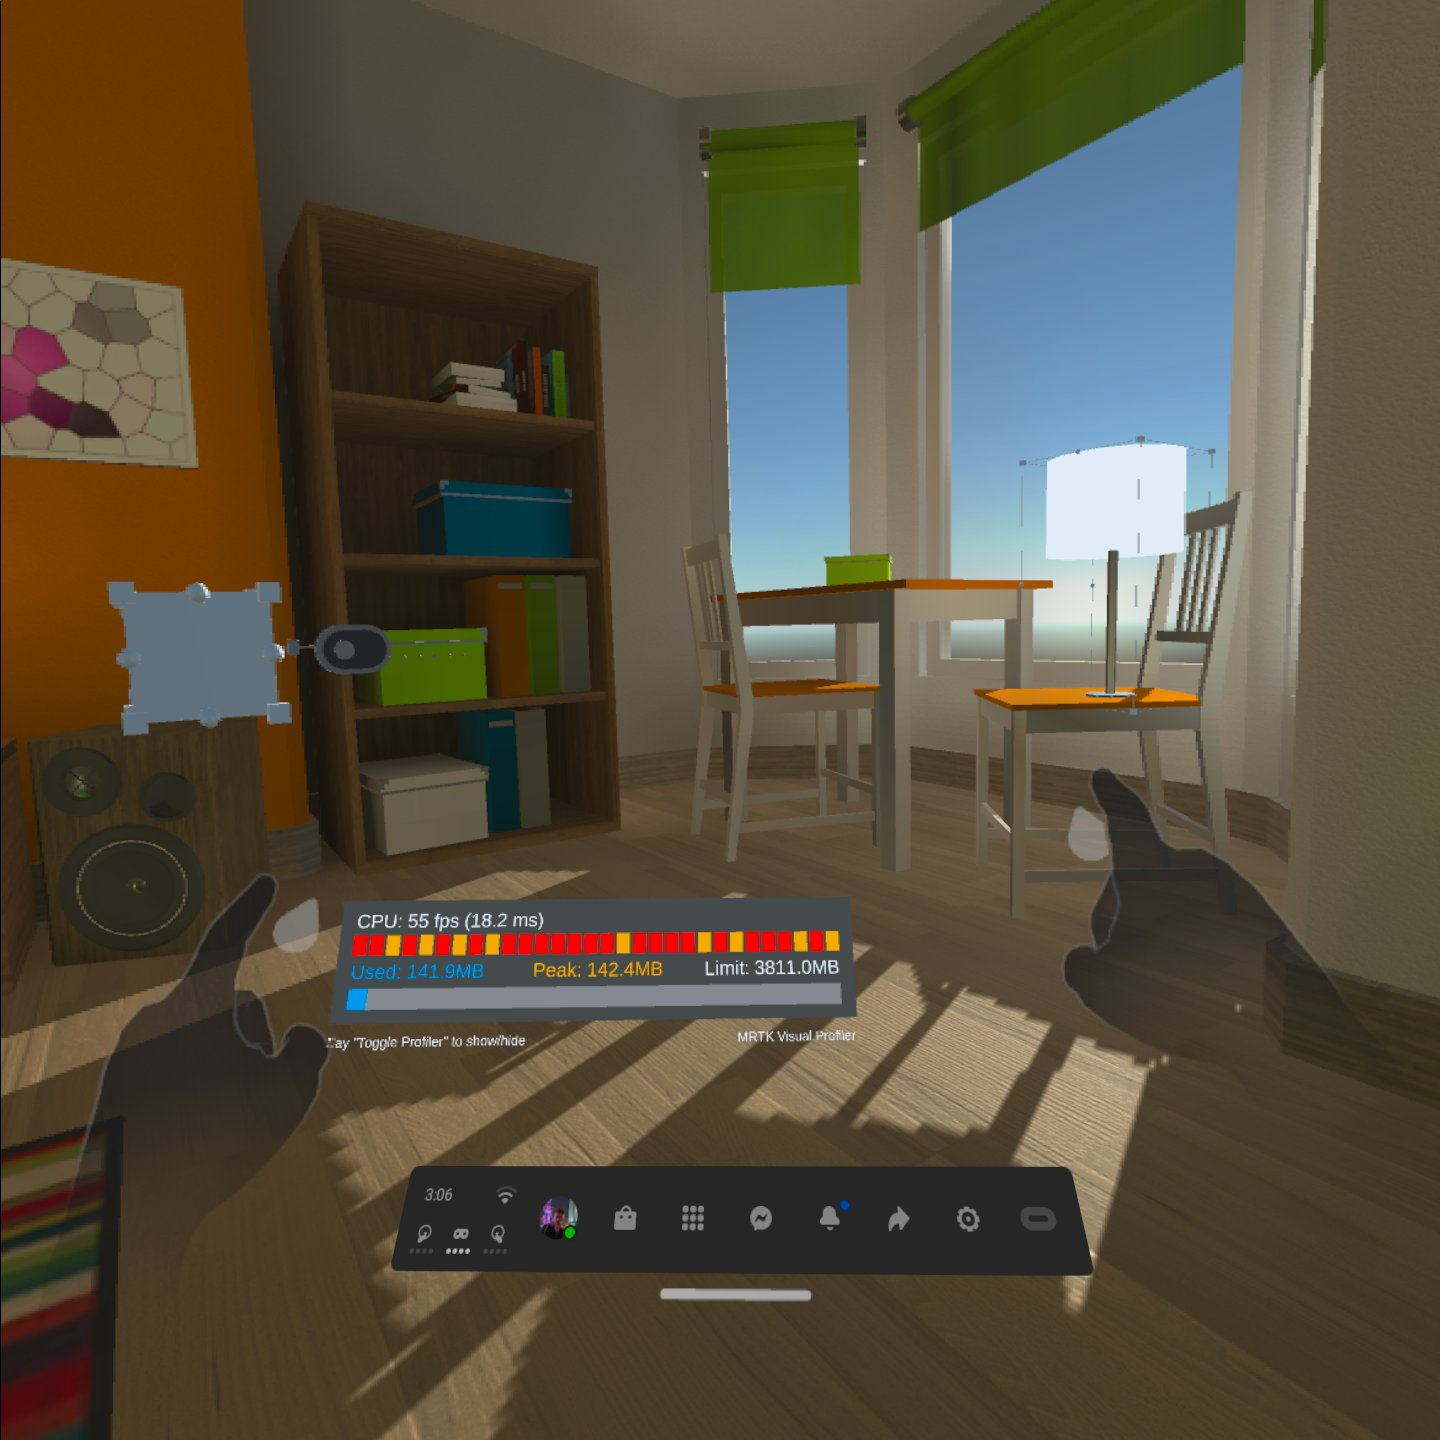
\includegraphics[width=0.45\linewidth]{figures/Series2FPSOculus.jpg}}
  \caption{Screenshots of the experiment.}
  \label{fig:exp-screenshot}
\end{figure}

\begin{figure}
  \centering
  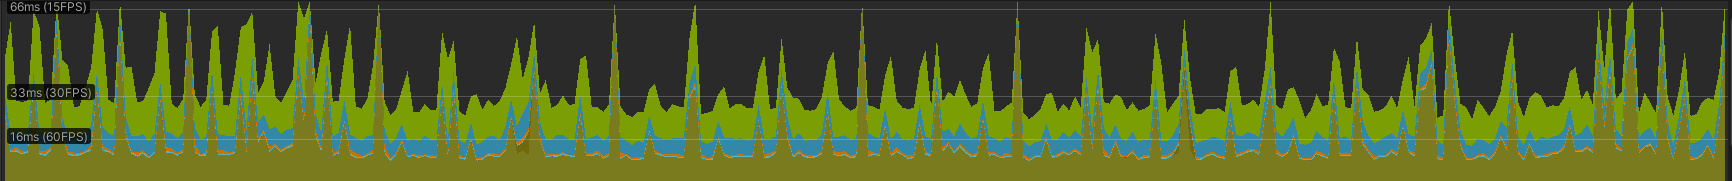
\includegraphics[width = 0.9 \linewidth]{figures/Series2FPSpng.png}
  \caption{FPS graph during the first series of the experiment of computations transfer.}
  \label{fig:Series2FPSpng-figure}
\end{figure}

\begin{figure}
  \centering
  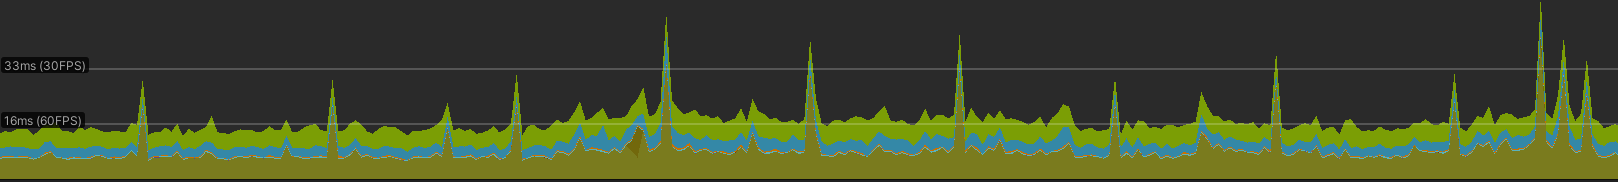
\includegraphics[width = 0.9 \linewidth]{figures/Series1FPS.png}
  \caption{FPS graph during the second series of the experiment of computations transfer.}
  \label{fig:Series1FPSpng-figure}
\end{figure}

Considering that gesture recognition is processed no more than once per frame, it significantly influenced the user experience, resulting in a big $t_{\Delta}$. The frequency of gesture value retrieval can be called polling rate. When a polling rate is 1000Hz, the gesture position is retrieved only once per frame (Table~\ref{tab:polling-rate-table}). Probably, there is a linear dependency on the time spent on performing the test and the polling rate during the test.

\begin{table}
  \centering
  \begin{threeparttable}[c]
    \caption{Polling rate to response time of gesture recognition dependence}
    \label{tab:polling-rate-table}
    \begin{tabular}{ll}
      \toprule
      Polling rate, Hz    & Response time, ms                 \\
      \midrule
      72Hz & 13.9ms \\
      65Hz & 15.4ms \\
      20Hz & 50ms \\
      10Hz & 100ms \\
      \bottomrule
    \end{tabular}
  \end{threeparttable}
\end{table}

However, the experiment's main challenge was to show how transferring resource-intensive computing from a VR headset to a server improves user experience, significant for the VR-IoT Research platform. Thus, the experiment can be considered successful.\footnote{Please note that this experiment cannot be considered scientifically substantiated since the number of tests and the number of participants is small. In addition, it is impossible to control the external factors that add random error, such as system optimization that affects the stability of the frame rate, room lighting that affects the accuracy of hand recognition, the size of the participants' hands, and the participants' experience with virtual reality systems. As a result, the reproduction of this experiment is almost impossible. Nevertheless, this experiment serves as an example of the requirement to transfer resource-intensive computing from the VR headset to the server.
}


In the next experiment, the author proved that it is possible to work together in one VR-IoT environment by adding new IoT devices to the system and changing their parameters:
\begin{enumerate}
    \item The time for adding a device to the system is limited by the performance of a specific platform and the speed of the Internet connection within the Wi-Fi network. When running 300 sequential ping tests from remote PC to localhost PC, all the values ​​obtained were less than 100ms, with 90 percent values ​​ranging from 45ms to 70ms. The time spent by the device on creating widgets for a smart vacuum cleaner roughly corresponded to the time of system initialization;
    \item Time interval from changing an Item on the remote PC to updating the widgets on localhost PC did not exceed 60ms.
\end{enumerate}

Thus, the speed of the network plays a significant role in the operation of the system. The minimal network latency available now in Wi-Fi 6 networks and 6G networks in the future can significantly improve the simultaneous work inside the same VR-IoT environment. However, it has been observed that operations such as adding new devices to the system will remain time-consuming. Since there is a request to create game objects for each of the Item's widgets, the author assumes that the main delay is associated precisely with the internal processes inside the Unity 3D engine.

The next chapter shows how the VR-IoT research platform developers can theoretically work around these limitations.
% !TeX root = ../thuthesis-example.tex

\chapter{THEORETICAL EVALUATION OF VR-IOT RESEARCH PLATFORM}

A theoretical assessment of the platform's various parameters is provided in this chapter. Compared to the existing solutions on the market, this is the first solution to automatically add any device from the real world to Virtual reality. Also, the platform allows researchers to create new devices in Virtual reality through the Things designer. Even though this research's main goal was to design the platform, the API for external projects connected to the platform will also be presented. The limitations dictated by hardware were considered in the previous chapter. In this chapter, the limitations dictated by the architecture are discussed.

A functional solution for IoT research requires support for various types of devices. Although the IoT market has numerous different devices, general types of device parameter values ​​can be specified. Following the definitions given in Chapter 3, each device is represented as a Thing and includes several Items. Thus, each device existing or created in the future can be divided into blocks in terms of the VR-IoT Research Platform architecture. The supported Item types are listed in the Table~\ref{tab:items-table}.

\begin{table}
  \centering
  \begin{threeparttable}[c]
    \caption{The supported Item types}
    \label{tab:items-table}
    \begin{tabular}{ll}
      \toprule
      ITEM TYPE    &         DESCRIPTION                 \\
      \midrule
      Color &	RGB Color value \\
      Contact & Whether the sensors are located close enough to each other \\
      DateTime & Date and time parameters \\
      Dimmer &	Dimmer value in percentage \\
      Group &	An Item containing other Items \\
      Image &	The binary data of an image \\
      Location & GPS Coordinates \\
      Number & Value stored in number format \\
      Number:<dimension> & Number Item with specified unit support \\
      Player & Item that control video, audio playback \\
      String &	Text or binary data \\
      Switch & Boolean value \\
      \bottomrule
    \end{tabular}
  \end{threeparttable}
\end{table}

The universal Item is String since the data collected by IoT sensors can be represented in binary format in almost all cases. Hence, the data operated by IoT devices can be placed inside Item blocks.

After NUIX-Studio App receives the Item of a specific format, the Semantic model is updated. Next, the Item corresponding Widgets are updated as well.

\section{Widgets support}

The platform provides only basic Widgets for the Items. These Widgets are used to give an example of how to visualize the IoT devices' data. Researchers can create Widgets specific to the device they develop using the NUIX-Studio API.

However, in most cases, researchers can save time by using the basic Widgets. Several Widgets based on the Mixed Reality Toolkit (\cite{MRTK2021}), such as Color Picker, Pinch Slider, Switcher and Button, were developed. Light-connected, Player-, Location- and Group-based Widgets were developed without using Mixed Reality Toolkit.

\section{Things designer}

Thanks to using a block structure to represent devices, researchers can change various parameters of existing devices by changing specific blocks and create new devices by combining the blocks. This action is possible in a tool called Things designer. This tool is described in detail below.

The Semantic model is visualized inside the Web interface. Researchers can assign Widgets for each of the Items and group the Items together. After the setup is completed, researchers can further develop new devices inside the NUIX-Studio App. Next, they can create new Widgets inside VR and connect them to the existing Items. The position for each of the Widgets is added to the Semantic model as an Item. Having set the widget's position and other parameters, the user can exit the application on a device and then continue research using a different device or analyze the items' data stored on the server. Since changes in Items values are periodically written to the server, they can be visualized by the built-in system tools (Figure~\ref{fig:PersistenceExample-figure}) or further analyzed using external frameworks providing useful insights. In addition, NUIX-Studio App also allows the creation of not only Widgets but also Items.

\begin{figure}
  \centering
  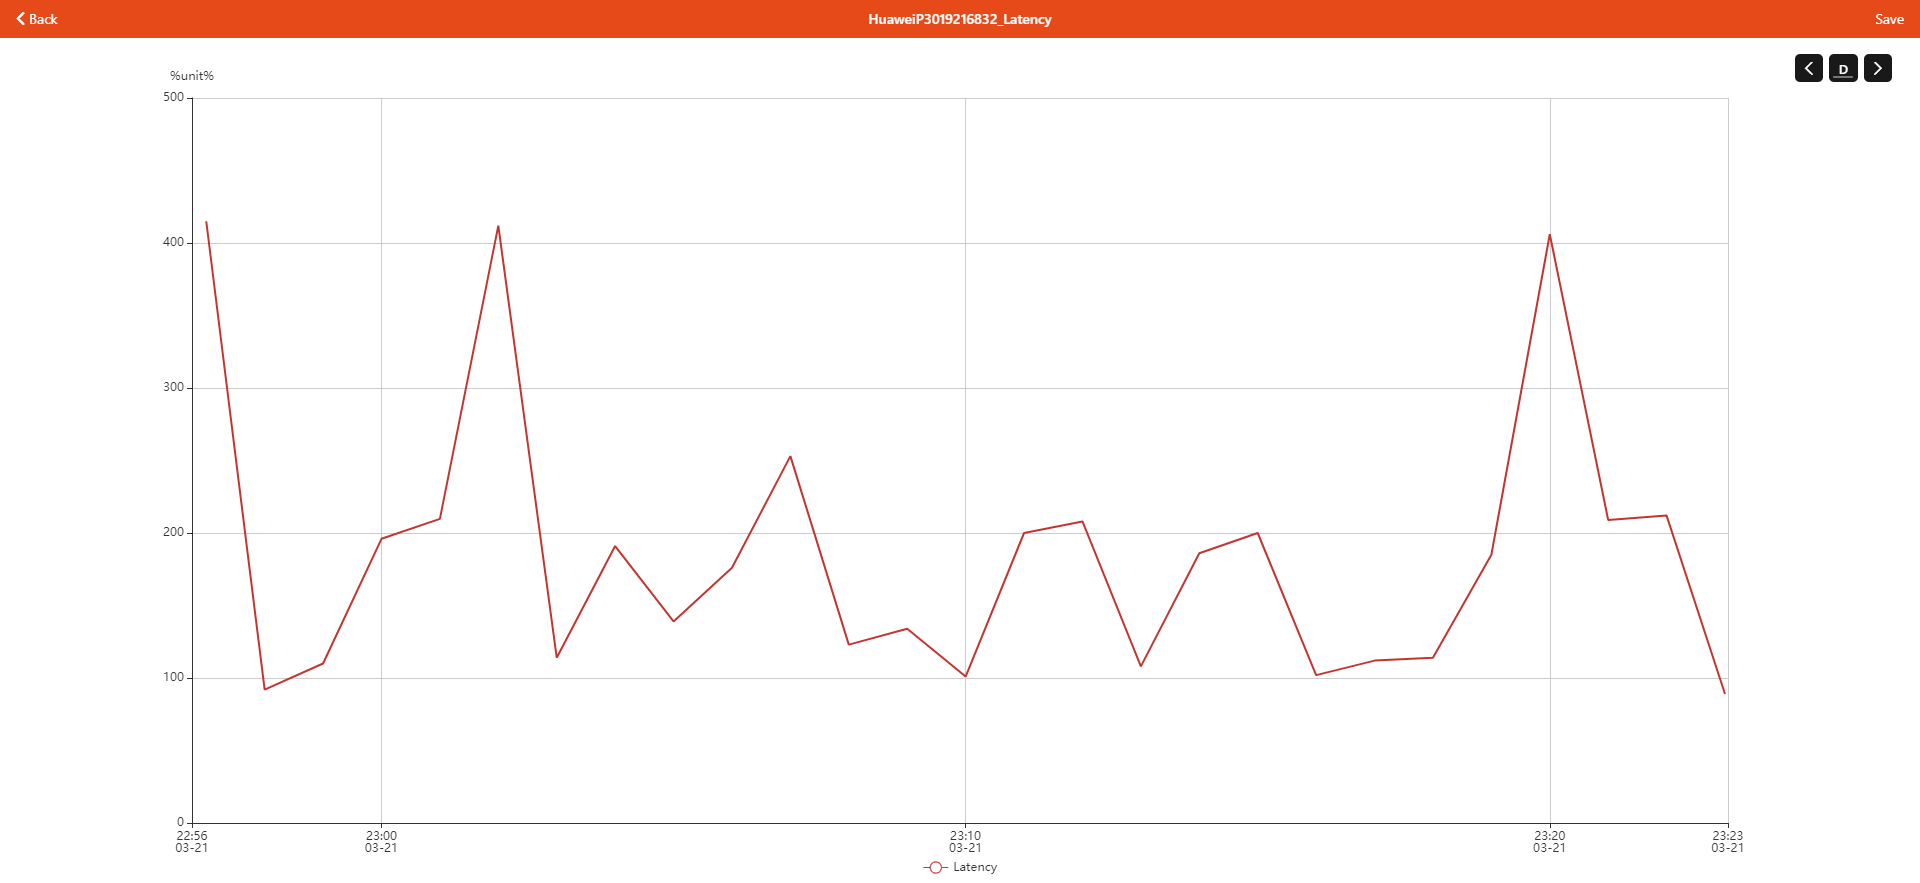
\includegraphics[width=0.9\linewidth]{figures/PersistenceExample.png}
  \caption{Persistence example: Latency value for accessing a remote device (in ms). }
  \label{fig:PersistenceExample-figure}
\end{figure}

\section{Device visualization and real-virtual world location mapping}

Each of the IoT devices is visualized through Widgets, but Widgets' designing by 3D modeling requires additional time. If a 3D model of the device already exists, the researcher can add it to the platform as a Widget and then connect extra widgets to it.

In the used IoT environment, not every device has a corresponding 3D model. There are several solutions to this problem. The first solution is to use 3D models of similar devices. However, it is not always possible to find the particular model, or the quality of these models does not meet the requirements. The second solution is device scanning. With the help of 3D scanners based on depth cameras, it is already possible to scan things with acceptable accuracy, especially at a relatively affordable price. If millimeter precision scanning is required, then expensive professional solutions can be used.

The resulting Widgets of 3D models are added to virtual reality. In the case of the NUIX-Studio App, scenes representing different environments are used. Scenes can be created within Unity editor and using Things designer by interpreting the surrounding objects as Widgets (for example, people's position on the street is represented as an Item of Location type). This approach takes quite a long time to construct a scene, especially if there is a need to use a copy of the real environment in Virtual reality. To reduce the simulation time, researchers can use solutions such as 3D scanning the environment. It is possible to scan the environment with good accuracy on many different smartphones using Depth Lab from Google and with excellent accuracy on the iPhone 12 Pro using Apple ARKit. However, these scans of the environment are static scenes. If an object inside this environment is moved, then the scan will have to be performed again. Unfortunately, there is currently no solution to this problem. However, in the next chapter, it will be shown that the platform can be adapted to work with augmented reality, thus eliminating the need to match the real world with the virtual one fully.

Various devices can track the movement of real IoT devices in the real world, such as Bluetooth tags, QR codes, magnetic field sensors, etc. Researchers can use API to change the position of each widget. Thus, when the device's position in the real world changes, the device's Widgets position in the virtual world will also change. Besides, it is possible to perform the opposite action, but this requires a device that will move IoT devices in the real world.

\section{Physics support}

With the transfer of resource-intensive calculations to a separate server, it becomes possible to perform more reliable physical object simulations. Computations such as processing light, sound, and electromagnetic waves of other frequencies and various substances such as gas, water, are only limited by existing algorithms.

\section{Scalability}

When the number of Widgets within the system increases, platform performance remains at an acceptable level. Because each Widget is assigned some unique id, the time it takes to access a specific Widget is O(1) operations. Event processing time takes O(n) operations, where n is the number of connected widgets. It is theoretically impossible to reduce the complexity of processing an event since every Widget has to be accessed. In this case, the event processing time is linearly dependent on the number of Widgets connected to the Item. In general, the platform's overall performance also linearly depends on the number of IoT devices in the environment.

\section{Conclusion}

Thus, it was shown that the platform's architecture allows support of all possible devices, creation of new devices from existing ones, and placing them in the virtual world. The platform enables the efficient processing of requests from an unlimited number of devices.

However, the platform's architecture does not circumvent the limitations associated with some theoretical calculations. Yet, in order to get around these limitations, researchers can use the platform inside Augmented reality, which is discussed in more detail in the next chapter.
% !TeX root = ../thuthesis-example.tex

\chapter{SUMMARY, DISCUSSION AND FUTURE DIRECTIONS}

\section{Discussion and future directions}

Оригинальность работы состоит в том, что не существует исследований на тему создания и взаимодействия устройств для VR-IoT окружения, все исследователя концентрируются именно на управлении IoT устройствами с помощью шлемов виртуальной реальности.
Автор надеется продолжить работу над платформой в будущем уже в лаборатории университета. Остановимся подробнее на дальнейших этапах разработки, предложенных автором.

\begin{figure}
  \centering
  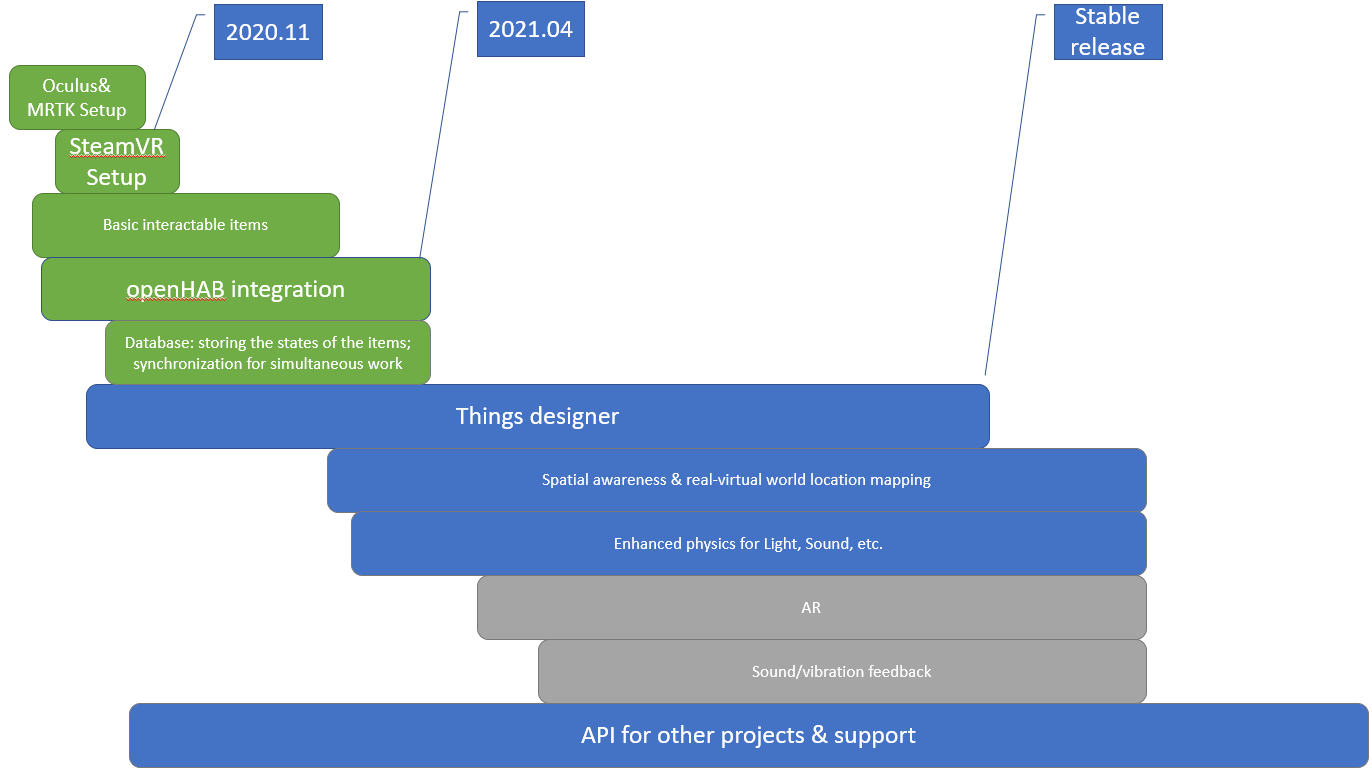
\includegraphics[width=0.9\linewidth]{figures/Timeline.png}
  \caption{Timeline}
  \label{fig:Timeline-figure}
\end{figure}

As seen in (Figure~\ref{fig:Timeline-figure}), the development started from providing support for Virtual reality headsets. Следующий шагом была реализация поддержки openHAB и базы данных для одновременной работы в одной среде. В тексте данной работы обсуждалось, что данные две задачи можно считать выполненными. Тем не менее, разработку Things designer пока на данный момент считать завершенной нельзя, так как необходимо дальнейшее исследование, to provide a bigger variety of supported Widgets and Items.

Mixed Reality toolkit can provide real-world environmental awareness for apps running on Hololens. It is already possible to run NUIX-Studio APP on Hololens, although, it has not yet been tested. Using spatial awareness, it will be possible to align virtual Widgets onto IoT devices. Developing real-virtual world location mapping for the Widgets for Virtual reality will be needed as well.

Currently, only advanced illumination can be computed on the NUIX-Studio APP. Researchers may need more accurate data to create new IoT devices. In this case Unity Game Engine can be extended with more accurate light, sound and other physics support.

Providing AR support requires adding new interactions techniques, as well as training Deep learning models to provide object recognition. Researchers can use both AR and VR to research on new IoT devices, with AR being responsible for retrieving the coordinates of the devices from the real world (by OpenCV, Tensoflow Graphics, etc.), and VR for visualizing environments that are difficult or impossible to show in AR (for example, flying on a plane or driving a car).

Augmented reality, Virtual reality and Mixed Reality are not the only interfaces to interact with IoT. What if the feedback from IoT devices only by sound and vibrations is provided? NUIX-Studio can be adapted for such limitations. One of the example usages of this approach is a research for visually impaired people in IoT environment.

Во время всего цикла разработки должен разрабатываться API для встраивания внешних разработок в платформу, в том числе проектов студентов HCI Lab.

\section{Summary}

Цель работы выполнена: представлена платформа для создания новых устройств для существующего IoT мира в виртуальной реальности, помогающая создавать новые устройства. Показано, что она позволяет это выполнить как теоретически, так и практически.



% 其他部分
\backmatter

% 参考文献
% References
\bibliography{ref/refs}  % 参考文献使用 BibTeX 编译
% \printbibliography       % 参考文献使用 BibLaTeX 编译

% 附录
% Appendix
\appendix
% Appendix

\chapter{USE IN EXTERNAL PROJECTS}

You can include in this section important evidence that is related to your research, but might affect the logic of your main thesis if included in the main writing. E.G. tables, pseudo-code, graphs etc. You can add accordingly.
附录是与论文内容密切相关、但编入正文又影响整篇论文编排的条理和逻辑性的资料,例如某些重要的数据表格、计算程序、统计表等,是论文主体的补充内容,可根据需要设置。

% Appendix figures
\section{Figure example 图表示例}

% Below is an example of inserting an appendix image
\subsection{Figure 图}

This is an example of an appendix image: (Figure~\ref{fig:appendix-figure})
附录中的图片示例(图~\ref{fig:appendix-figure})。

\begin{figure}
  \centering
  \includegraphics[width=0.6\linewidth]{example-image-a.pdf}
  \caption{Example of appendix figure 附录中的图片示例}
  \label{fig:appendix-figure}
\end{figure}

% Tables
\subsection{Tables 表格}

Below is an example of tables in the appendix (Table~\ref{tab:appendix-table}).

附录中的表格示例(表~\ref{tab:appendix-table})。

\begin{table}
  \centering
  \caption{附录中的表格示例}
  \begin{tabular}{ll}
    \toprule
    % Input the file + description here
    % File name & Description
    文件名          & 描述                         \\
    \midrule
    thuthesis.dtx   & 模板的源文件,包括文档和注释 \\
    thuthesis.cls   & 模板文件                     \\
    thuthesis-*.bst & BibTeX 参考文献表样式文件    \\
    thuthesis-*.bbx & BibLaTeX 参考文献表样式文件  \\
    thuthesis-*.cbx & BibLaTeX 引用样式文件        \\
    \bottomrule
  \end{tabular}
  \label{tab:appendix-table}
\end{table}


% This is an example of mathematical formula
\section{Mathematical formula 数学公式}

This is an example of formula (Equation~\eqref{eq:appendix-equation})
附录中的数学公式示例(公式~\eqref{eq:appendix-equation})。
\begin{equation}
  \frac{1}{2 \symup{\pi} \symup{i}} \int_\gamma f = \sum_{k=1}^m n(\gamma; a_k) \mathscr{R}(f; a_k)
  \label{eq:appendix-equation}
\end{equation}
% % !TeX root = ../thuthesis-example.tex

% PLEASE IGNORE THIS PART! This is not applicable to Master students




\begin{survey}
\label{cha:survey}

\title{Title of the Survey}
\maketitle


\tableofcontents


本科生的外文资料调研阅读报告。


\section{Figures and Tables}

\subsection{Figures}

An example figure in appendix (Figure~\ref{fig:appendix-survey-figure}).

\begin{figure}
  \centering
  \includegraphics[width=0.6\linewidth]{example-image-a.pdf}
  \caption{Example figure in appendix}
  \label{fig:appendix-survey-figure}
\end{figure}


\subsection{Tables}

An example table in appendix (Table~\ref{tab:appendix-survey-table}).

\begin{table}
  \centering
  \caption{Example table in appendix}
  \begin{tabular}{ll}
    \toprule
    File name       & Description                                         \\
    \midrule
    thuthesis.dtx   & The source file including documentaion and comments \\
    thuthesis.cls   & The template file                                   \\
    thuthesis-*.bst & BibTeX styles                                       \\
    thuthesis-*.bbx & BibLaTeX styles for bibliographies                  \\
    thuthesis-*.cbx & BibLaTeX styles for citations                       \\
    \bottomrule
  \end{tabular}
  \label{tab:appendix-survey-table}
\end{table}


\section{Equations}

An example equation in appendix (Equation~\eqref{eq:appendix-survey-equation}).
\begin{equation}
  \frac{1}{2 \symup{\pi} \symup{i}} \int_\gamma f = \sum_{k=1}^m n(\gamma; a_k) \mathscr{R}(f; a_k)
  \label{eq:appendix-survey-equation}
\end{equation}


\section{Citations}

Example citations in appendix.
\cite{abrahams99tex}
\cite{salomon1995advanced}
\cite{abrahams99tex,salomon1995advanced}


\bibliographystyle{unsrtnat}
\bibliography{ref/appendix}

\end{survey}
       % 本科生:外文资料的调研阅读报告
% % !TeX root = ../thuthesis-example.tex

\begin{translation}
\label{cha:translation}

\title{书面翻译题目}
\maketitle

\tableofcontents


本科生的外文资料书面翻译。


\section{图表示例}

\subsection{图}

附录中的图片示例(图~\ref{fig:appendix-translation-figure})。

\begin{figure}
  \centering
  \includegraphics[width=0.6\linewidth]{example-image-a.pdf}
  \caption{附录中的图片示例}
  \label{fig:appendix-translation-figure}
\end{figure}


\subsection{表格}

附录中的表格示例(表~\ref{tab:appendix-translation-table})。

\begin{table}
  \centering
  \caption{附录中的表格示例}
  \begin{tabular}{ll}
    \toprule
    文件名          & 描述                         \\
    \midrule
    thuthesis.dtx   & 模板的源文件,包括文档和注释 \\
    thuthesis.cls   & 模板文件                     \\
    thuthesis-*.bst & BibTeX 参考文献表样式文件    \\
    thuthesis-*.bbx & BibLaTeX 参考文献表样式文件  \\
    thuthesis-*.cbx & BibLaTeX 引用样式文件        \\
    \bottomrule
  \end{tabular}
  \label{tab:appendix-translation-table}
\end{table}


\section{数学公式}

附录中的数学公式示例(公式~\eqref{eq:appendix-translation-equation})。
\begin{equation}
  \frac{1}{2 \symup{\pi} \symup{i}} \int_\gamma f = \sum_{k=1}^m n(\gamma; a_k) \mathscr{R}(f; a_k)
  \label{eq:appendix-translation-equation}
\end{equation}


\section{文献引用}

文献引用示例\cite{abrahams99tex}。


% 书面翻译的参考文献
\bibliographystyle{unsrtnat}
\bibliography{ref/appendix}

% 书面翻译对应的原文索引
\begin{translation-index}
  \nocite{salomon1995advanced}
  \bibliographystyle{unsrtnat}
  \bibliography{ref/appendix}
\end{translation-index}

\end{translation}
  % 本科生:外文资料的书面翻译

% 致谢
% Acknowledgements
% !TeX root = ../thuthesis-example.tex
% Acknowledgements
\begin{acknowledgements}

  I would like to express my deepest appreciation to my supervisor Professor Yu Chun, advisor Yan Yukang for the perpetual support of my research, Thank you for suggestions, advice and contribution. Your guidance assisted me in all the time of this research.
  
  I would also like to extend my deepest gratitude to Professor Shi for sharing their your knowledge and insights. 
  
  I thank my fellow lab mate Qian Yanlin and Jessy for the stimulating discussions, feedback, and cooperation.
  
  This work would not have been possible without the partnership and support from the faculty, staff, and students of Tsinghua University, Computer Science Department, HCI Lab. 
  
  I am grateful to all the people I was unable to meet in person who committed to NUIX and NUIX-Studio in particular.
  
\end{acknowledgements}


% 声明
% Statement
\statement
% 生成的声明页是否要插入页眉和页脚(默认 empty)
% 仅在需要进行电子签名时,才需要打开这一选项
% 插入的扫描声明页总是会生成页眉(研究生)和页脚,不受这一选项影响
% \statement[page-style=plain]
% 将签字扫描后的声明文件 scan-statement.pdf 替换原始页面
% \statement[file=scan-statement.pdf]

% 个人简历、在学期间完成的相关学术成果
% Resume
% !TeX root = ../thuthesis-example.tex

\begin{resume}

  %\section*{Resume}
  % Please note the empty line to ensure the correct format for this section.
    Fedor Ivachev was born on 10th October 1997 in Moscow, Russia.
    
    He began his bachelor's study in the Department of Computational Mathematics and Cybernetics, Lomonosov Moscow State University in September 2015, majoring in Applied Mathematics and Computer Science, and got a Bachelor of Computer Science and Software Engineering in June 2019.
    
    He started to pursue a master's degree in Computer Science  and Technology in the Department of Computer Science and Technology, Tsinghua University since September 2019.

\end{resume}


% 指导教师/指导小组学术评语
% Comments from the supervisor or reviewers
% !TeX root = ../thuthesis-example.tex

\chapter{COMMENTS FROM THESIS SUPERVISOR}

该论文面向物联网环境中交互系统开发的需求,研发了一套虚实结合的开发和验证系统。该系统基于虚拟现实构建,将物理环境中的信息设备与虚拟世界中的设备连接起来,提供了数据同步和交换的机制,使得开发人员可以在虚拟环境中快速构建交互场景,实验交互技术,并进行初步用户实验。该系统进而允许将虚拟设备替换为真实的物理设备,并且物理设备的状态改变也能引起虚拟设备状态的变化,从而实现虚实融合的交互系统开发。该方法可以有效提升开发效率,已经应用在了清华大学的数门课程中,初步验证了该系统的有效性。

% 答辩委员会决议书
% Decision of the defense committee
% !TeX root = ../thuthesis-example.tex

\chapter{RESOLUTION OF THESIS DEFENSE COMMITTEE}

This thesis proposes...

The language of this section should be in concordance with the original document (either Chinese or English)

论文提出了……

论文取得的主要创新性成果包括:

1. ……

2. ……

3. ……

论文工作表明作者在×××××具有×××××知识,具有××××能力,论文××××,答辩××××。

答辩委员会表决,(×票/一致)同意通过论文答辩,并建议授予×××(姓名)×××(门类)学博士/硕士学位。


% 本科生的综合论文训练记录表(扫描版)
% \record{file=scan-record.pdf}

\end{document}
